\documentclass[a4paper,11pt]{book} %ADD diffusion OR archiv for final versions
% \usepackage[latin9]{inputenc}
\usepackage[T1]{fontenc}    % Output encoding: allows proper hyphenation and accents
\usepackage[utf8]{inputenc} % Input encoding: allows typing é, è, ñ, etc.
\usepackage{lmodern}        % Scalable fonts with full T1 support
\usepackage{xspace}			  
\usepackage[english]{babel}
\usepackage[margin=28mm,includeheadfoot]{geometry}
% width fig 149mm!!!
\usepackage{thcover}
\usepackage{physics}
\usepackage{setspace}
\usepackage{amssymb}
\usepackage{float}
\usepackage{caption} % Load caption before minitoc
\usepackage{setspace}
\usepackage{mathtools}
\usepackage{tikz}
\usepackage{gensymb}

\usepackage[backend=biber,style=numeric,sorting=none,backref=true]{biblatex}
\addbibresource{./bib/bib_these.bib}
\addbibresource{./bib/references.bib}
\addbibresource{./bib/references_these.bib}
% \addbibresource{./bib/library_these.bib}
% \addbibresource{./bib/optomechanics.bib}
% \addbibresource{./bib/quantum.bib}


\onehalfspacing % or \singlespacing or \doublespacing
\input{./preamb/preamb-graph.tex}
\input{./preamb/preamb-math.tex}
\input{./preamb/preamb-util.tex}
\usepackage{hyperref}
\hypersetup{
    colorlinks=true,
    linkcolor=black,
    filecolor=magenta,      
    urlcolor=blue,
    pdftitle={My Thesis Title},
    pdfauthor={Author Name},
    pdfsubject={Thesis Subject},
    pdfkeywords={keyword1, keyword2, keyword3},
}
\usepackage{minitoc}
\renewcommand{\thechapter}{\Roman{chapter}}
\renewcommand{\thefigure}{\thechapter.\arabic{figure}} % Figure numbering: Chapter.Figure
\renewcommand{\thetable}{\thechapter.\arabic{table}}   % Table numbering: Chapter.Table
\dominitoc
\raggedbottom
\begin{document}
% Ensure consistent and flat minitoc spacing (uses titletoc
% Patch minitoc internal spacing

%%%%%%%%%%%%%%%%%%%%%%%%%%%%%% PAGES LIMINAIRES %%%%%%%%%%%%%%%%%%%%%%%%%%%%%%%
\frontmatter
%!TeX encoding = UTF-8
% Metadata for coverpages
\thesisname{Thèse de doctorat}
\gradename{docteur}
\univ{de l’université Pierre et Marie Curie}
\logos{upmc}{}{tintin}                   % Un à trois logo. Le 1er est celui de \univ
\specialite{Physique}
\ecoledoctnum{564}
\ecoledoct{Physique en Île-de-France}
\title{La laine des Dupondt au \og Pays de l'or noir\fg}
\titleen{Dupondt's wool in  ``Land of Black Gold’’}

% si nécessaire, pour les métadonnées
%\titlemeta{La laine des Dupondt au Pays de l'or noir} 
%\titlemetaen{Dupondt's wool in "Land of Black Gold" } 

\date{1\up{er} avril 1999}
\author{Eugène TRIBOULET}
\advisor{Tryphon TOURNESOL}
\atinstitution{à l’École normale supérieure}
\atlab{{\Large au Laboratoire de tintinologie théorique et appliquée}}
% Jury as LaTeX Tabular. Pas de président avant soutenance								  
\jury{ %                         
M. & Séraphin LAMPION & Rapporteur        \\
M. & Alfredo TOPOLINO & Rapporteur        \\
M. & Fan SE-YENG  & Examinateur           \\
M\up{me}& Bianca CASTAFIORE & Examinatrice \\
M. & Tryphon TOURNESOL & Directeur de thèse }

\makeatletter
\@ifpackageloaded{thcover-psl}{\logos{PSL}{tintin}{}}{\relax}
\makeatother

\resume{Lorem ipsum dolor sit amet, consectetur adipiscing elit. Nulla elit ipsum, hendrerit in
congue at, sodales at nunc. Cras luctus venenatis arcu faucibus ultrices. Etiam nisi est, sollicitudin
quis efficitur non, faucibus at elit. Mauris lacinia posuere efficitur. Duis sit amet sollicitudin ligula.
Donec auctor facilisis neque eget sollicitudin. Vivamus at pharetra turpis.
Aliquam feugiat porta purus, et porta libero. Morbi mollis luctus purus, et lacinia odio auctor
eget. Cum sociis natoque penatibus et magnis dis parturient montes, nascetur ridiculus mus.
Maecenas condimentum at urna ut malesuada. Pellentesque ut pharetra elit, id ultricies quam. Ut
cursus, metus sit amet rhoncus tempor, arcu elit tristique ipsum, rutrum pretium massa risus nec
massa. Sed congue lacus mauris, sit amet lobortis nunc mattis eget. Vestibulum fermentum felis
dictum leo hendrerit facilisis id id nibh. Nunc et ornare nunc. Donec pellentesque porta tellus,
fermentum euismod risus gravida pharetra. Suspendisse potenti. In lobortis, ipsum ut viverra
feugiat, sem nunc ullamcorper enim, et volutpat nisi libero id sem. Maecenas vestibulum nibh sit
amet nulla placerat euismod. Fusce aliquet condimentum justo, non porttitor sem volutpat non.
Aenean id diam et sem bibendum imperdiet at ut enim. Integer non porttitor nunc.
Suspendisse potenti. Integer sed ultricies odio, a pellentesque ligula. Suspendisse maximus ma-
lesuada egestas. Vestibulum quis commodo tellus, et tincidunt lectus. Praesent vehicula, velit
eu molestie eleifend, metus orci dictum dui, bibendum ultricies augue lacus vestibulum dui. Ut
vestibulum lorem eros, non cursus leo dignissim sit amet. \par\hfill  (1700 car max, espaces inclus)}
\motscles{Pétrole, additif, Emirats, Dupond, Dupont }

% si nécessaire, pour les métadonnées
%\titlemetaen{Dupondt's wool in "Land of Black Gold" } 

\abstract{ Pellentesque sollicitudin tortor sit amet justo pulvinar posuere. Nullam aliquet felis
vitae arcu fringilla iaculis. Suspendisse at nisl at orci porta mattis sit amet in velit. Vestibulum
mattis aliquam massa, interdum facilisis metus fermentum nec. Donec venenatis leo ut egestas
scelerisque. Nam vel diam mi. Vestibulum eros purus, ullamcorper id quam et, interdum elemen-
tum odio. Suspendisse at velit erat. Phasellus mattis accumsan nibh id aliquet.
Etiam id interdum lectus. Vestibulum tempor non mauris at vestibulum. Proin rutrum ullamcor-
per lectus, vitae suscipit justo ultrices et. Nullam fringilla, dolor lacinia viverra dignissim, felis
velit luctus enim, ut feugiat augue ante eget dui. Mauris consequat, diam ac hendrerit rutrum,
arcu turpis sagittis neque, vulputate lacinia lorem odio eu mi. Ut lobortis bibendum diam at
cursus.
Pellentesque libero augue, mollis in hendrerit in, rutrum vel dolor. Mauris sollicitudin sit amet
nisl nec suscipit. Vestibulum pretium odio lobortis ipsum elementum, ut aliquam neque rutrum.
Vivamus at sapien in elit pretium venenatis quis ac tellus. Suspendisse dictum ornare blandit.
Nam vitae orci nec nulla luctus commodo non id est. Integer sit amet purus vitae purus malesuada
dictum. Suspendisse luctus diam magna, eu dapibus nisi ultrices nec. Nullam sed suscipit risus.
Mauris congue id dui ac aliquet. Sed luctus mauris sed faucibus viverra. Donec lectus odio,
aliquam a mi sit amet, pharetra mattis magna. Cras mattis tristique vehicula. Mauris nulla
tortor, consequat ac viverra at, dignissim at quam. Donec eget accumsan turpis, quis iaculis
turpis.
\par\hfill (1700 chars max, spaces included)}
\keywords{Oils, additive, emirate,  Dupond, Dupont }
 % Ensure this file is correctly filled
\frontcover\ % requires thcover.sty loaded and thcoverdata.tex filled
\chapter*{Remerciements}
    \par
    Merci bien  
\
\begingroup
\setstretch{1.8} % or \singlespacing, \onehalfspacing, etc.
\tableofcontents
\endgroup % \chapter*{Introduction to the thesis}
 
 % At the end of the 19th century, the first optical cavity was realised by Alfred Perot and Charles Fabry using two thinly silvered plane glass plates set accurately parallel. The successive reflections of light inside the cavity interfering with each other create sharp resonance peak and it was rapidly clear that this new type of interferometer could be used to perform very precise interferometric measurement. 
 



  Intro intro
 
 





\mainmatter\ 
\chapter*{Introduction}\label{chap:intro}
\addcontentsline{toc}{chapter}{Introduction} % ensures it appears in the main TOC
\mtcaddchapter

\section*{Historical background}
\addcontentsline{toc}{section}{Historical background} % ensures it appears in the main TOC


\section*{State of the art}
\addcontentsline{toc}{section}{State of the art} % ensures it appears in the main TOC



\section*{Relevance of this work}
\addcontentsline{toc}{section}{Relevance of this work} % ensures it appears in the main TOC
 
\newcommand{\adag}[1]{\hat{a}_{#1}^\dagger}
\newcommand{\aop}[1]{\hat{a}_{#1\vphantom{\dagger}}}
\chapter{Theory: Background}
This chapter will cover the elementary concepts required to describe an membrane based optomechanical system in a quantum regime. We will first recall basics on optical field quantization as well describing coherent and squeezed light field, to then turn to the more specific frequency dependent squeezed light field. Secondly, we will cover the mathematical description of a mechanical resonator interacting with a generic coherent optical field, highlighting the differences with the seminal optomechanical system of a mirror on a spring. Finally, we will derive the equations of motions of a membrane based optomechanical system with frequency dependent squeezed optical fields. 
\minitoc
\newpage
\section{Quantum Optics}
\subsection{Quantum Description of Light}

\subsubsection{Quantised Electromagnetic Field}
% \the\textwidth
We consider the quantised electromagnetic field in a volume $V$. The electric field operator can be written as  
\begin{equation}
\hat{\mathbf{E}}(\mathbf{r}, t) 
= i \sum_{\ell} \mathcal{E}_\ell 
\left[ \hat{a}^{\vphantom{\dagger}}_{\ell}\,\mathbf{f}_{\ell}(\mathbf{r})\,e^{-i\omega_{\ell} t} 
- \hat{a}_{\ell}^\dagger\,\mathbf{f}_{\ell}^*(\mathbf{r})\,e^{+i\omega_{\ell} t} \right],
\end{equation}
where   $\mathcal{E}_l = \sqrt{\frac{\hbar \omega_l}{2 \varepsilon_0 V}}$ is the field amplitude per photon in mode $\ell$, $\hbar$ is the reduced Planck constant, $\omega_\ell$ is the angular frequency of mode $\ell$, and $\varepsilon_0$ is the vacuum permittivity. The spatial mode functions $\mathbf{f}_{\ell}(\mathbf{r})$ form an orthonormal basis in $V$ according to  
\begin{equation*}
\int_V d^3r\; \mathbf{f}_{\ell}^*(\mathbf{r}) \cdot \mathbf{f}_{\ell'}(\mathbf{r}) 
= \delta_{\ell \ell'} .
\end{equation*}
The annihilation and creation operators $\hat{a}_{\ell}(t)$ and $\hat{a}_{\ell}(t)^\dagger$ satisfy the canonical commutation relations  
\[
[\hat{a}_{\ell}^{\vphantom{\dagger}}, \hat{a}_{\ell'}^\dagger] = \delta_{\ell \ell'} \,, \quad
[\hat{a}_{\ell}^{\vphantom{\dagger}}, \hat{a}_{\ell'}^{\vphantom{\dagger}} ] = 0, \quad [\hat{a}_{\ell}^\dagger, \hat{a}_{\ell'}^\dagger] = 0  
\]
The explicit time dependence of the operators allows one to describe both slow classical modulations of the field and the intrinsic quantum fluctuations.

\subsubsection{Fock basis}
In this description of the optical field, each mode $\ell$ is modeled as a quantum harmonic oscillator with a discrete set of energy eigenstates known as \textit{Fock states} or number states, denoted $\ket{n_\ell}$. These states form an orthonormal basis and satisfy $\hat{n}_{\ell} \ket{n_\ell} = n_\ell \ket{n_\ell}$, where $\hat{n}_{\ell}$ is the number operator defined by
\[
\hat{n}_{\ell} = \hat{a}_{\ell}^\dagger \hat{a}^{\vphantom{\dagger}}_{\ell}.
\]
The action of the creation and annihilation operators on these states is given by
\[
\hat{a}^{\vphantom{\dagger}}_{\ell} \ket{n_\ell} = \sqrt{n_\ell} \ket{n_\ell - 1}, \quad
\hat{a}_{\ell}^\dagger \ket{n_\ell} = \sqrt{n_\ell + 1} \ket{n_\ell + 1}.
\]
They allow transitions between Fock states by lowering or raising the photon number in mode $\ell$ by one unit. The vacuum state $\ket{0_\ell}$ is annihilated by $\hat{a}^{\vphantom{\dagger}}_{\ell}$, satisfying $\hat{a}^{\vphantom{\dagger}}_{\ell} \ket{0_\ell} = 0$. Thus, the Hamiltonian for the electromagnetic field becomes a sum of harmonic oscillator energies:
\begin{equation}
\hat{H} = \sum_\ell \hbar \omega_{\ell} \, \hat{a}_{\ell}^\dagger \hat{a}^{\vphantom{\dagger}}_{\ell} 
\end{equation}
where we ignore the constant zero-point energy term $\frac{1}{2} \hbar \omega_{\ell}$ for simplicity. \\

In the following parts, we will always focus on a single mode of the electromagnetic field unless stated otherwise (for the mode matching part), which is sufficient to illustrate the concepts of quantum optics and optomechanics. The generalization to multiple modes is straightforward and follows the same principles. The electrif field operator is then written
\begin{equation}
\hat{\mathbf{E}}(\mathbf{r}, t)
= i \mathcal{E}_0
\left[ \hat{a}^{\vphantom{\dagger}}\,\mathbf{f}(\mathbf{r})\,e^{-i\omega_0 t}
- \hat{a}^\dagger\,\mathbf{f}^*(\mathbf{r})\,e^{+i\omega_0 t} \right].
\end{equation}


\subsubsection{Quadrature Operators}
We describe the phase-space properties of a field mode using hermitian quadrature operators. These are linear combinations of the annihilation and creation operators that correspond to measurable observables in the electromagnetic field. The two most common quadratures are defined as follows:
\begin{equation}
\mathbf{\hat{a}}\;\equiv\;
\begin{pmatrix}\hat a_1\\[2pt]\hat a_2\end{pmatrix}
=\mathbf\Gamma \, \mathbf{\hat{u}}, \label{II.2}
\qquad
\mathbf \Gamma \equiv
\begin{pmatrix}
1 & 1 \\
-i & i
\end{pmatrix},
\quad
\mathbf{\hat{u}}\;\equiv\;
\begin{pmatrix}\hat a\\ \hat a^\dagger\end{pmatrix}
\end{equation}
where we defined the field vector $\mathbf{\hat{u}}$ and the transfer matrix $\mathbf \Gamma$, later used to switch from One-Photon to Two-Photon description of optical elements. In components, we then have $\hat a_1=\hat a^\dagger+\hat a$ and $\hat a_2=i(\hat a^\dagger-\hat a)$.
The matrix form commutator reads
\begin{equation}
[\mathbf{\hat{u}}, \mathbf{\hat{u}}^{\dagger}] = \mathbf{\sigma_z}, 
\end{equation}
with $\sigma_z$ the Pauli Z matrix. 
An arbitrary rotated quadrature pair is obtained by
\begin{equation}
\mathbf{\hat{a}_\phi}\;\equiv\;
\begin{pmatrix}\hat a_\phi\\[2pt]\hat a_{\phi+\pi/2}\end{pmatrix}
= \mathbf R(\phi)\,\mathbf{\hat{a}}
= \mathbf R(\phi)\,\mathbf\Gamma \,\mathbf{\hat{u}},
\qquad
 \mathbf R(\phi)\equiv
\begin{pmatrix}
\cos\phi & \sin\phi \\
-\sin\phi & \cos\phi \label{II.4}
\end{pmatrix}.
\end{equation}
We notice than 
\begin{equation}
\mathbf R(\phi)\,\boldsymbol{\Gamma}
=
\begin{pmatrix}
\cos\phi & \sin\phi \\
-\sin\phi & \cos\phi
\end{pmatrix}
\begin{pmatrix}
1 & 1 \\
-i & i
\end{pmatrix}
=
\begin{pmatrix}
e^{-i\phi} & e^{i\phi} \\[4pt]
-\,i\,e^{-i\phi} & \;\;i\,e^{i\phi}
\end{pmatrix}.
\end{equation}
so that in components we have 
\begin{equation}
\begin{alignedat}{3}
\hat a_\phi \;&=\;& \hat a_1 \cos\phi + \hat a_2 \sin\phi \;&= \hat a\,e^{-i\phi} + \hat a^\dagger\,e^{+i\phi}\\
\hat a_{\phi+\pi/2} \;&=\;& -\hat a_1 \sin\phi + \hat a_2 \cos\phi \;&= i\!\left(\hat a^\dagger\,e^{+i\phi} - \hat a\,e^{-i\phi}\right).
\end{alignedat}
\end{equation}
The commutators of the rotated quadrature operators read
\begin{equation}
\begin{aligned}
[\hat{\mathbf{a}}_\phi , \hat{\mathbf{a}}_\phi^{\dagger}]
&= \mathbf R(\phi) \mathbf \Gamma\,[\hat{\mathbf{u}},\hat{\mathbf{u}}^{\dagger}]\, \mathbf \Gamma^{\dagger} \mathbf R^{\dagger}(\phi) \\[4pt]
&= \mathbf R(\phi)\mathbf \Gamma \mathbf \sigma_z \mathbf \Gamma^{\dagger} \mathbf R^{\dagger}(\phi) \\[4pt]
&= 2i\, \mathbf R(\phi) \mathbf J \mathbf R^{\dagger}(\phi) \\[4pt]
&= 2i\,\mathbf J,
\end{aligned}
\end{equation}
where $\mathbf{J}$ is the symplectic form defined as
\begin{equation}
\mathbf{J} \equiv
\begin{pmatrix}
0 & 1 \\
-1 & 0
\end{pmatrix}.
\end{equation}
Note that since $\hat{\mathbf{a}}_\phi$ is hermitian, we have $\hat{\mathbf{a}}_\phi^\dagger = \hat{\mathbf{a}}_\phi^T$, and similarly $\mathbf{R^\dagger(\phi)} = \mathbf{R}^T(\phi)$ since all its entries are real. \\ 
\\
This compact vector form will be used later for the One- and Two-Photon description of the light field behaviours in optomechanical systems with squeezed light input. \\
\noindent \textbf{Note:} \color{red} notes the fact that these are defined for a specific $\ell$, so at each mode is associated such a quadrature vector. The multimode treatment is used by the multimode quantum optics community, notably to describe mutimode non gaussian states, hidden squeezing (beyond homodyne detection correlations, Patera and co) \color{black}
\subsubsection{Linearization of the optical field}

The annihilation operator can be decomposed as
\begin{equation}
\begin{split}
    \hat{a} & = \langle \hat{a} \rangle + \delta\hat{a}\\
    & = \bar{\alpha} + \delta\hat{a} \\
\end{split}
\label{II.8}
\end{equation}
where \(\langle \hat{a} \rangle = \bar{\alpha} \in \mathbb{C}\) is the mean complex amplitude of the quantum state, and \(\delta\hat{a}\) represents quantum fluctuations with \(\langle \delta\hat{a}\rangle = 0\). Note this decomposition is valid for any quantum state, including coherent and squeezed states. We note $\bar{\alpha}$ to distinguish it from the complex amplitude $\alpha$ of a coherent state introduced below, which is a specific case of this decomposition. The associated matrix form is 
\begin{equation}
\mathbf{\hat{u}} =  \begin{pmatrix} \bar{\alpha}  \\ \bar{\alpha}^*  \end{pmatrix} + \begin{pmatrix} \delta\hat{a} \\ \delta\hat{a}^\dagger \end{pmatrix} =  \mathbf{\bar{u}} + \mathbf{\delta \hat{u}}
\end{equation}
and it then follows that fluctuations in the quadrature operators can be expressed as
\begin{equation}
  \mathbf{\delta \hat{a}_\phi} = \mathbf{R}(\phi) \, \mathbf\Gamma  \, \mathbf{\delta \hat{u}}
\end{equation}
They also retain the canonical commutation relations
\begin{equation}
[\mathbf{\delta \hat{u}}, \mathbf{\delta \hat{u}}^{\dagger}] = \mathbf{\sigma_z} \qquad \Rightarrow \qquad
[\mathbf{\delta \hat{a}_\phi}, \mathbf{\delta \hat{a}_\phi}^{T}] = 2i\,\mathbf{J}.
\label{II.11}
\end{equation}

\noindent \textbf{Note:} \color{red} notes on first and second moments, as well as beyond second moments correlations and their use i.e. when and why is this linearization ok to use etc etc \color{black}

\subsubsection{Heisenberg Uncertainty Relation }
The covariance of Hermitian operators \(\hat{A}\) and \(\hat{B}\) is defined as
\begin{equation}
    \mathrm{Cov}(\hat{A},\hat B) = \tfrac12 \big\langle \{ \delta\hat{A}, \delta\hat{B} \} \big\rangle \\
\end{equation}
Now if $\hat{A}=\hat{B}$ this is the variance written as 
\begin{equation}
    \Delta A^2 = \langle {(\delta \hat{A})^2} \rangle
\end{equation}
Considering the quadrature operators, we define the covariance matrix as
\begin{equation}
\mathbf{V_\phi} \equiv \tfrac12 \big\langle \{  \mathbf{\delta \hat{a}_\phi},  \mathbf{\delta \hat{a}_\phi}^{\,T} \} \big\rangle
= \begin{pmatrix}
\Delta \hat{a}_\phi^2 &
\mathrm{Cov}(\hat{a}_\phi,\hat{a}_{\phi+\pi/2}) \\[4pt]
\mathrm{Cov}(\hat{a}_\phi,\hat{a}_{\phi+\pi/2})  &
\Delta \hat{a}_{\phi+\pi/2}^2
\end{pmatrix}
\end{equation}
and the Heisenberg uncertainty relation reads as
\begin{equation}
  \det \mathbf{V_\phi} \geq 1 \qquad \Rightarrow \qquad \Delta \hat{a}^2_\phi \Delta \hat{a}^2_{\phi+\pi/2} - \mathrm{Cov}^2(\hat{a}_\phi,\hat{a}_{\phi+\pi/2})\geq 1
\end{equation}

\subsection{Coherent and Squeezed States}
We now turn to standard optical quantum states, in particular gaussian states i.e.\ full positive in Wigner function representations such as coherent and squeezed states, that we will denote in braket notation as $|\alpha\rangle$ and $|\alpha,r, \theta\rangle $.
\subsection*{Coherent States:}
The coherent state $\ket{\alpha}$ is an eigenstate of the annihilation operator:
\begin{equation}
\hat{a}\ket{\alpha} = \alpha \ket{\alpha}
\label{II.14}
\end{equation}
where $\alpha = |\alpha| e^{i\bar{\varphi}}$ is a complex number representing the mean coherent amplitude. In this notation, the angle $\bar{\varphi}$ is the mean angle of the distribution, used to describe the relative phase to a reference (e.g. a local oscillator). The $\hat{a}$ linear decomposition above (Eq~\eqref{II.8}) then yields $\alpha = \bar{\alpha}$ for a coherent state. It can be expressed in the Fock basis as
\begin{equation}
\ket{\alpha} = e^{-|\alpha|^2/2} \sum_{n=0}^\infty \frac{\alpha^n}{\sqrt{n!}}\,\ket{n}
\label{II.15}
\end{equation}
and are generated by the action of the displacement operator $\hat{D}(\alpha)$ on the vacuum state $\ket{0}$:
\begin{equation}
\ket{\alpha} = \hat{D}(\alpha)\ket{0},\qquad \hat{D}(\alpha) = \exp\!\left(\alpha \hat{a}^\dagger - \alpha^* \hat{a}\right)
\label{II.16}
\end{equation}
\noindent \textbf{Note:} \color{red} note on the convention used i.e. $\alpha \neq \bar{\alpha}$, $\alpha_0 \neq \bar{\alpha}_0$ \color{black}
\subsubsection*{Expectation values of quadrature operators}

Using the quadrature vector $\hat{\mathbf a} = (\hat{a}_1,\,\hat{a}_2)^T = \Gamma (\hat{a}, \hat{a}^\dagger)^T$ given in Eq~\eqref{II.2}, the expectation values in a coherent state are
\begin{equation}
\langle \hat{\mathbf a} \rangle
= \Gamma
\begin{pmatrix}\alpha\\ \alpha^*\end{pmatrix}
= \begin{pmatrix}
\alpha+\alpha^* \\[2pt]
i(\alpha^*-\alpha)
\end{pmatrix}
= 2\begin{pmatrix}
\mathrm{Re}\,\alpha \\[2pt]
\mathrm{Im}\,\alpha
\end{pmatrix}.
\label{II.CS.1}
\end{equation}
For a quadrature rotated by an angle $\phi$ (Eq~\ref{II.4}),
\begin{equation}
\langle \hat{\mathbf a}_\phi\rangle
= \mathbf R(\phi)\,\langle \hat{\mathbf a}\rangle
=
2\begin{pmatrix}
\mathrm{Re}\big(\alpha e^{-i\phi}\big) \\[2pt]
\mathrm{Im}\big(\alpha e^{-i\phi}\big)
\end{pmatrix}.
\end{equation}


\subsubsection*{Amplitude and phase quadratures}

It is convenient to introduce the amplitude-phase quadrature vector at $\phi = \bar{\varphi}$
\begin{equation}
\hat{\mathbf a}_{\bar{\varphi}} =
\begin{pmatrix}
\hat{p} \\[2pt]
\hat{q}
\end{pmatrix}
=
\begin{pmatrix}
\hat{a}_{\bar{\varphi}} \\[2pt]
\hat{a}_{\bar{\varphi}+\pi/2}
\end{pmatrix}.
\end{equation}
with expectation values
\begin{equation}
\langle \hat{\mathbf a}_{\bar{\varphi}} \rangle
=
2\begin{pmatrix}
|\alpha| \\[2pt]
0
\end{pmatrix},
\end{equation}



\subsubsection*{Covariance matrix}
For a coherent state, fluctuations are vacuum-like:
\begin{equation}
\Delta \hat{a}_\phi^2 = \Delta \hat{a}_{\phi+\pi/2}^2 = 1,
\qquad
\mathrm{Cov}(\hat{a}_\phi,\hat{a}_{\phi+\pi/2}) = 0,
\end{equation}
so that
\begin{equation}
\mathbf V_\phi =
\begin{pmatrix}
1 & 0\\
0 & 1
\end{pmatrix}
= \mathbb{I}_2,
\quad \forall \phi .
\label{II.CS.3}
\end{equation}
This saturates the Heisenberg uncertainty relation $\det \mathbf V_\phi = 1$ in the units defined here i.e. it is a minimum uncertainty state. 

\subsubsection*{Photon number statistics}

The mean and variance of the photon number operator $\hat{N}=\hat{a}^\dagger\hat{a}$ are
\begin{equation}
\langle \hat{N} \rangle = |\alpha|^2,
\qquad
\Delta N^2 = |\alpha|^2.
\label{II.19}
\end{equation}
That is, coherent states display Poissonian photon statistics.


\begin{figure}
\centering
\includegraphics[width=\textwidth]{./chap2/fig/quantum_states.pdf}
\caption{Phase-space representations of quantum states and transformations.
(a) Wigner function of the vacuum state: a circular Gaussian centered at the origin, representing equal quantum fluctuations in both quadratures $a_1$ and $a_2$.
(b) Wigner function of a coherent state: a displaced circular Gaussian, showing a shift in phase space along an angle $\varphi$ with unchanged, isotropic noise.
(c) Wigner function of a squeezed vacuum state: an elliptical Gaussian centered at the origin, with reduced noise along a rotated quadrature $X_\theta$ and increased noise in the orthogonal direction.
(d) Wigner function of a displaced squeezed state: an ellipse shifted away from the origin, combining anisotropic fluctuations and a nonzero mean amplitude. The displacement angle $\varphi$ and squeezing angle $\theta$ are independent.} 
\end{figure}


\subsection*{Squeezed States:}

Squeezed states $|\alpha, r, \theta\rangle $ are quantum gaussian states of light in which the noise (variance) of one quadrature is reduced below the vacuum level, at the expense of increased noise in the conjugate quadrature. The single-mode squeezed vacuum state is defined as
\begin{align}
|0, r, \theta \rangle = \hat{S}(r, \theta) |0\rangle , \quad \hat{S}(\theta) = \exp\left[\frac{r}{2}(e^{-2 i\theta} \hat{a}^2 - e^{-2 i\theta} \hat{a}^{\dagger 2})\right]
\end{align}
where $r$ is the squeezing parameter (strength) and $\theta$ is the squeezing angle i.e. the angle along which one quadrature is reduced below vacuum level. The most general Gaussian state is the displaced squeezed state, obtained by applying both the squeezing operator $\hat{S}(r, \theta)$ and the displacement operator $\hat{D}(\alpha)$ to the vacuum:
\begin{equation}
|\alpha, r, \theta\rangle = \hat{S}(r, \theta)\hat{D}(\alpha)|0\rangle
\end{equation}
where $\hat{D}(\alpha)$ displaces the state in phase space by the complex amplitude $\alpha$, defined similarly to the coherent state. \\

\noindent \textbf{Note:}  The displacement and squeezing operators do not commute, i.e. $\hat{D}(\alpha)\hat{S}(r, \theta) \neq \hat{S}(r, \theta)\hat{D}(\alpha)$. However, both orderings correspond to experimentally valid procedures: one can either squeeze the vacuum and then displace (e.g. by mixing with a coherent state ona beamsplitter), or squeeze a coherent state straight away (e.g. by seeding an optical parametric amplifier). The resulting state is always a displaced squeezed state, but the relative phase between displacement and squeezing may differ.
% -------------------------------------------------
\subsubsection*{Expectation values of quadrature operators}

Using the usual quadratures defined in Eq~\eqref{II.2} and \eqref{II.4}, the expectation values in a displaced squeezed state are
\begin{equation}
\langle \mathbf{\hat{a}} \rangle
= 2
\begin{pmatrix}
\mathrm{Re}\,\alpha \\[2pt]
\mathrm{Im}\,\alpha
\end{pmatrix}, 
\qquad
\langle \mathbf{\hat{a}_\phi} \rangle
= 2
\begin{pmatrix}
\mathrm{Re}\!\left(\alpha e^{-i\phi}\right) \\[2pt]
\mathrm{Im}\!\left(\alpha e^{-i\phi}\right)
\end{pmatrix}.
\label{II.xx3}
\end{equation}
For a squeezed vacuum ($\alpha=0$) all quadrature means vanish.

\subsubsection*{Quadrature aligned with the squeezing axis \color{red} to rewrite \color{black}}

Choosing $\phi = \theta$ yields
\begin{equation}
\Delta \hat a_\theta^2 = e^{-2r}, \qquad
\Delta \hat a_{\theta+\pi/2}^2 = e^{2r}, \qquad
\mathrm{Cov}(\hat a_\theta, \hat a_{\theta+\pi/2}) = 0,
\end{equation}
with uncertainty product $\Delta \hat a_\theta\, \Delta \hat a_{\theta+\pi/2} = 1$ saturating the Heisenberg bound.
The corresponding mean vector is
\begin{equation}
\langle \mathbf{\hat{a}_\theta} \rangle
= 2
\begin{pmatrix}
\mathrm{Re}(\alpha e^{-i\theta}) \\[2pt]
\mathrm{Im}(\alpha e^{-i\theta})
\end{pmatrix}.
\label{II.xx7}
\end{equation}

\begin{figure}
\centering
\includegraphics[width=\textwidth]{./chap2/fig/quantum_quadraturesBis.pdf}
\caption{Phase-space representations of quantum states and transformations.
(a) Wigner function of the vacuum state: a circular Gaussian centered at the origin, representing equal quantum fluctuations in both quadratures $X_1$ and $X_2$.
(b) Wigner function of a coherent state: a displaced circular Gaussian, showing a shift in phase space along an angle $\varphi$ with unchanged, isotropic noise.
(c) Wigner function of a squeezed vacuum state: an elliptical Gaussian centered at the origin, with reduced noise along a rotated quadrature $X_\theta$ and increased noise in the orthogonal direction.
(d) Wigner function of a displaced squeezed state: an ellipse shifted away from the origin, combining anisotropic fluctuations and a nonzero mean amplitude. The displacement angle $\varphi$ and squeezing angle $\theta$ are independent.} 
\end{figure}
% -------------------------------------------------
\subsubsection*{Covariance matrix}

Let $\psi \equiv \phi - \theta$ be the measurement angle $\phi$ relative to the squeezing axis $\theta$.  
For a displaced squeezed state, the covariance matrix is
\begin{equation}
\mathbf{V}_\phi = \mathbf R(\psi)
\begin{pmatrix}
e^{-2r} & 0 \\[2pt]
0 & e^{2r}
\end{pmatrix}
\mathbf R(\psi)^{T}.
\label{II.xx4}
\end{equation}
Expanding this explicitly gives
\begin{equation}
\mathbf{V}_\phi =
\begin{pmatrix}
e^{-2r} \cos^2\!\psi + e^{2r} \sin^2\!\psi 
& \frac{1}{2} \sin 2\psi \,\left(e^{2r} - e^{-2r}\right) \\[6pt]
\frac{1}{2} \sin 2\psi \,\left(e^{2r} - e^{-2r}\right) 
& e^{-2r} \sin^2\!\psi + e^{2r} \cos^2\!\psi
\end{pmatrix}.
\label{II.xx5}
\end{equation}
The covariance term is therefore
\begin{equation}
\mathrm{Cov}(\hat a_\phi, \hat a_{\phi+\pi/2})
= \frac{1}{2} \sin 2(\phi-\theta)\, \left(e^{2r} - e^{-2r}\right),
\label{II.xx6}
\end{equation}
which vanishes when $\sin 2(\phi-\theta) = 0$, i.e.
\begin{equation*}
\phi - \theta \in \left\{ 0, \frac{\pi}{2}, \pi, \ldots \right\}.
\end{equation*}
Along these principal axes of squeezing, $\mathbf{V}_\phi$ is diagonal. 

\subsubsection{Amplitude and Phase squeezed states}
Considering a displaced squeezed state, two special cases are of interest: the amplitude squeezed state where $\theta=\bar{\varphi}$ and the phase squeezed state where $\theta = \bar{\varphi}+\pi/2$. In the first case, the amplitude quadrature $\hat{p}$ is squeezed, while the phase quadrature $\hat{q}$ is anti-squeezed. In the second case, the phase quadrature is squeezed, while the amplitude quadrature is anti-squeezed. The covariance matrices for these states can be derived from Eq.~\eqref{II.xx4} by setting $\psi = 0$ or $\psi = \pi/2$, respectively.
\subsubsection*{Photon number statistics}

The mean and variance of the photon number operator $\hat N = \hat a^\dagger \hat a$ in a displaced squeezed state are
\begin{equation}
\langle \hat N \rangle = |\alpha|^2 + \sinh^2 r,
\qquad
\Delta N^2 = |\alpha|^2 \cosh 2r + \frac{1}{2} \sinh^2 2r.
\label{II.xx8}
\end{equation}
\color{red}
to rewrite
\color{black}
This shows that the squeezing operation increases the mean photon number of the coherent state by adding photons. Physically, this reflects the fact that generating squeezed light requires injecting energy into the system, so the squeezed vacuum contains correlated field excitations (photons) in even numbers. This is further seen by examining the photon-number distribution $P_n$: for a squeezed vacuum only even $n$ occur, while displacement progressively repopulates the odd $n$ and shifts weight to higher $n$, in agreement with the increase of $\langle \hat{N} \rangle$ and $\Delta N^2$ above.



\color{black}

\subsection{Sidebands and Quantum Noises}

\subsubsection{Modulation picture}
In realistic optical systems, the electromagnetic field is never perfectly monochromatic, nor isolated from its environment, nor static through time. Instead, it exhibits a finite spectral linewidth (stimulated emission, phase noise etc...), as well as non intentional/intentional modulations, all imprinted onto the carrier field. These effects cause the field amplitude and phase to evolve slowly compared to the optical frequency $\omega_0$. \\

As a result, the complex amplitude associated with each mode and described by the Schrodinger-picture annihilation operator $\hat{a}$, acquires an explicit time dependence beyond the standard fast-oscillating term $e^{-i\omega_0 t}$. It is often quoted as \textit{modulation} picture in the litterature. We then promote the field vector to 
\begin{equation}
\mathbf{\hat{u}}= \mathbf{\bar{u}} + \mathbf{\delta \hat{u}} \quad \rightarrow \quad
  \mathbf{\hat{u}}(t)=
 \mathbf{\bar{u}}(t) + \mathbf{\delta \hat{u}(t)}
\end{equation}
where the canonical commutation relations given in equation~\eqref{II.11} becomes:
\begin{equation}
  [\delta\mathbf{\hat{u}}(t), \delta \mathbf{\hat{u}}(t')^{\dagger}] = \mathbf{\sigma_z} \, \delta (t-t').
\end{equation}
This time dependence allows us to track both slow classical modulations of the field $\mathbf{\bar{u}}(t)$ and the intrinsic quantum fluctuations $\mathbf{\delta \hat{u}(t)}$. Note this is equivalent to the interaction picture where the reference angular frequency would be $\omega_0$, but where we also consider dynamical processes way slower than this frequency. Additionally, we will always consider the limit of weak fluctuations, where the quantum noise can be treated perturbatively around the classical field i.e. 
\[
|\bar{\alpha}(t)| \gg \Delta \hat a_\theta(t)
\]
The resulting field operator can then be expressed as a 
\begin{equation}
\begin{aligned}
\hat{\mathbf{E}}(\mathbf{r}, t) 
=i  \mathcal{E}_0 \bigg[ & \left[ \alpha(t)\, \mathbf{f}(\mathbf{r})\, e^{-i \omega_0 t} 
- \alpha^*(t)\, \mathbf{f}^*(\mathbf{r})\, e^{i \omega_0 t} \right] \\
\quad +  &\left[ \delta \hat{a}(t)\, \mathbf{f}(\mathbf{r})\, e^{-i \omega_0 t}
- \delta \hat{a}^\dagger(t)\, \mathbf{f}^*(\mathbf{r})\, e^{i \omega_0 t} \right] \bigg]
\end{aligned}
\end{equation} 

\subsubsection{Fourier Domain \& Sidebands}
To deal with noise spectra, we need to rewrite the various quadratures defined in the previous sections in the Fourier domain, where each frequency component is called a \textit{sideband}. The Fourier transform of the field vector is defined as
\begin{equation}
  \begin{split}
    \mathbf{\hat{u}}[\Omega] &= \frac{1}{\sqrt{2\pi}}\int_{\infty}^{-\infty}  dt \, e^{i\Omega t} \, \mathbf{\hat{u}}(t)\\
\mathbf{\hat{u}}(t) &= \frac{1}{\sqrt{2\pi}}\int_{\infty}^{-\infty}  d\Omega \, e^{-i\Omega t} \, \mathbf{\hat{u}}[\Omega]
  \end{split}
\end{equation}
where $\Omega \ll \omega_0$ is the sideband frequency relative to the so called \textit{carrier} frequency $\omega_0$. In this definition, a notable property is that the hermitian conjugate in the time domain translates to a frequency inversion in the Fourier domain:
\begin{equation}
   \Big[\hat{a}(t)\Big]^{\dagger} = \hat{a}^\dagger(t),  \quad
   \Big[\hat{a}[\Omega]\Big]^{\dagger}  = \hat{a}^\dagger[-\Omega].
\end{equation}
Carrying out the linearization in the Fourier domain, we have
\begin{equation}
  \begin{split}
      \mathbf{\hat{u}}[\Omega] &= \begin{pmatrix} \hat{a}[\Omega] \\ \hat{a}^\dagger[-\Omega] \end{pmatrix}  \\
       & = \begin{pmatrix} \bar{\alpha}[\Omega] \\ \bar{\alpha}^*[-\Omega] \end{pmatrix} + \begin{pmatrix} \delta\hat{a}[\Omega] \\ \delta\hat{a}^\dagger[-\Omega] \end{pmatrix} \\
      & = \mathbf{\bar{u}}[\Omega] + \mathbf{\delta \hat{u}}[\Omega]\\
  \end{split}
\end{equation}
with the fluctuations commutator reading
\begin{equation}
  [\delta \mathbf{\hat{u}}[\Omega], \delta \mathbf{\hat{u}}[\Omega']^{T}] = \mathbf{\sigma_z} \, \delta(\Omega + \Omega').
\end{equation}
This very way of writing the field vector is known as the \textit{two-photon} formalism, introduced by Caves and Schumaker~\cite{Caves1985,Caves1985a}. The quadrature operators in the Fourier domain are then written as 
\begin{equation}
  \begin{split}
      \mathbf{\hat{a}_\phi}[\Omega] &= \mathbf{R}(\phi) \, \mathbf{\Gamma} \, \mathbf{\hat{u}}[\Omega]\\
      & = \mathbf{R}(\phi) \, \mathbf{\Gamma} \,\mathbf{\bar{u}}[\Omega] + \mathbf{R}(\phi) \, \mathbf{\Gamma} \, \mathbf{\delta \hat{u}}[\Omega] \\
      & = \underbrace{2|\bar{\alpha}| \begin{pmatrix}
  \cos(\bar{\varphi}-\phi) \\[2pt]
  \sin(\bar{\varphi}-\phi)
\end{pmatrix} \delta(\Omega)}_{\text{classical part}} +
\underbrace{\mathbf{R}(\phi) \, \mathbf{\Gamma} \, \mathbf{\delta \hat{u}}[\Omega]}_{\text{quantum fluctuations}}
  \end{split}
\end{equation}


\noindent\textbf{Note: }
In the modulation picture, fluctuations in the time domain appear as symmetric sidebands at \(+\Omega\) and \(-\Omega\).
Any experimentally accessible, real signal arises from the interference of these two sidebands (quadratures in homodyne detection, intensity fluctuations, photocurrent spectra); equivalently, Hermiticity in time forces Fourier components to couple \(+\Omega\) with \(-\Omega\).
Packaging the field as the two-photon vector \(\big(\hat a[\Omega],\,\hat a^\dagger[-\Omega]\big)^{\mathsf T}\) therefore groups exactly the two degrees of freedom that generate a single measurable fluctuation at frequency \(\Omega\). This makes correlations between the sidebands (which are the essence of frequency-dependent squeezing) explicit and ensures that quadrature spectra remain manifestly real. By contrast, the vector \(\big(\hat a[\Omega],\,\hat a^\dagger[\Omega]\big)^{\mathsf T}\) is convenient for per-frequency photon-number or passive-scattering calculations, but it obscures the intrinsic pairing required to form real observables, forcing one to carry \(-\Omega\) separately.
For the noise-spectral analysis pursued here, the sideband-pair representation is thus the phenomenologically natural and algebraically minimal choice.


\subsubsection*{Amplitude Modulation (AM)}

Let the classical coherent amplitude be modulated at $\Omega_{\text{mod}}$ in amplitude:
\begin{equation}
  \alpha(t) = \bar{\alpha} \left(1 + \epsilon_a \cos(\Omega_{\text{mod}} t)\right)
\end{equation}
with $\epsilon_a \ll 1$, the field amplitude modulation depth. While the DC term lives at frequency $\omega_0$, the modulation introduces sidebands at frequencies $\omega_0 \pm \Omega_{\text{mod}}$, seen by expanding the cosine:
\begin{equation}
  \alpha(t) = \bar{\alpha} \Big( 1 + \frac{\epsilon_a }{2}\, e^{i\Omega_{\text{mod}} t} + \frac{\epsilon_a }{2} \,  e^{-i\Omega_{\text{mod}} t} \Big)
\end{equation}


\subsubsection*{Phase Modulation (PM)}
Let the classical coherent amplitude be modulated in phase at frequency $\Omega_{\mathrm{mod}}$:
\begin{equation}
\alpha(t) = \bar{\alpha} \, e^{i \epsilon_{\phi} \cos(\Omega_{\mathrm{mod}} t)}
\label{eq:PM_def}
\end{equation}
with $\epsilon_{\phi} \ll 1$ the field phase modulation depth. Expanding to first order in $\epsilon_{\phi}$ gives:
\begin{equation}
\alpha(t) \approx \bar{\alpha} \Big( 1 + \frac{i \epsilon_{\phi} }{2} \, e^{i\Omega_{\mathrm{mod}} t} + \frac{i \epsilon_{\phi} }{2} \, e^{-i\Omega_{\mathrm{mod}} t} \Big)
\label{eq:PM_expand}
\end{equation}
While the carrier term lives at frequency $\omega_0$, the modulation introduces sidebands at $\omega_0 \pm \Omega_{\mathrm{mod}}$, both shifted in phase by $\pi/2$ relative to the carrier.

\subsubsection{Linearized Hermitian Operators}
In both cases, the field contains a carrier at frequency $\omega$ and two sidebands at $\omega \pm \Omega$. Amplitude modulation results in sidebands that are in phase with the carrier, while phase modulation produces sidebands with a $\pm \pi/2$ phase shift relative to the carrier. We also note a general modulation process as :
\begin{equation}
\alpha(t) = \bar{\alpha} \left(1 + \varepsilon(t) \right)
\end{equation}
where $\varepsilon(t) \in \mathbb{C}$ is a modulation function that weakly modulates the complex amplitude in time, and that features information about the modulation frequency and depth. It then follows that the linearized amplitude-phase operators can be expressed as
\begin{equation}
\hat{\mathbf a}_{\bar{\varphi}} (t) = 2|\bar{\alpha}| \begin{pmatrix}
  1 \\ 0 
\end{pmatrix} + 2|\bar{\alpha}|\begin{pmatrix}
  \mathrm{Re}\big(\varepsilon(t) \big) \\
  \mathrm{Im}\big(\varepsilon(t) \big)
\end{pmatrix}
+ \begin{pmatrix}
  \delta \hat{p}(t) \\
  \delta \hat{q}(t)
\end{pmatrix}
\end{equation}

And the quadrature operators can be expressed as
\begin{equation}
\hat{\mathbf a}_{\bar{\varphi}} [\Omega] =2|\bar{\alpha}| \begin{pmatrix}
  1 \\ 0 
\end{pmatrix}\delta(\Omega) + 2|\bar{\alpha}|\begin{pmatrix}
  \mathrm{Re}\big(\varepsilon[\Omega] \big) \\
  \mathrm{Im}\big(\varepsilon[\Omega] \big)
\end{pmatrix}
+ \begin{pmatrix}
  \delta \hat{p}[\Omega] \\
  \delta \hat{q}[\Omega]
\end{pmatrix}
\end{equation}
Computing the Fourier transform for amplitude and phase modulations yields
\begin{equation}
  \begin{split}
    \varepsilon^{AM}(\Omega) & = \frac{\epsilon_a}{2} \Big(\delta(\Omega - \Omega_{\text{mod}}) +\delta(\Omega + \Omega_{\text{mod}}) \Big)\\
    \varepsilon^{PM}(\Omega) & = \frac{i\epsilon_\phi}{2} \Big(\delta(\Omega - \Omega_{\text{mod}}) + \delta(\Omega + \Omega_{\text{mod}})\Big)
  \end{split}
\end{equation}

\subsubsection{Noise Spectra}
We now define the cross spectra matrix for two arbitrary hermitian operators $\hat{A}$ and $\hat{B}$, which describes their correlations at different frequencies. It is defined as 
\begin{equation}
  \mathbf{S}_{AB}(\Omega) = \begin{pmatrix}
  S_{AA}(\Omega) & S_{AB}(\Omega) \\
  S_{BA}(\Omega) & S_{BB}(\Omega) 
  \end{pmatrix}
\end{equation}
where 
\begin{equation}
  2\pi \, \delta(\Omega + \Omega') \, S_{AB}(\Omega) = \frac{1}{2}\langle \{\hat{A}(\Omega),\,\hat{B}(\Omega') \} \rangle
\end{equation}

Computing 

\subsection{Two Photon Model }
We begin by recalling the quantized electric field operator for a single spatial mode with carrier frequency $\omega_0$ and mode function $\mathbf{f}(\mathbf{r})$ (as in Eq.~II.1):
\begin{equation}
\hat{\mathbf{E}}(\mathbf{r}, t) = i \mathcal{E} \left[ \hat{a}(t)\, \mathbf{f}(\mathbf{r})\, e^{-i \omega_0 t} - \hat{a}^\dagger(t)\, \mathbf{f}^*(\mathbf{r})\, e^{i \omega_0 t} \right]
\end{equation}
where $\hat{a}(t)$ is the slowly varying annihilation operator in the rotating frame.
To analyze the field in the sideband representation, we express the annihilation operator in terms of its Fourier components over positive frequencies:
\begin{equation}
\hat{a}(t) = \int_0^\infty \frac{d\omega}{2\pi} \, \hat{a}(\omega) e^{-i\omega t} 
\end{equation}
We introduce a central carrier frequency \( \omega_0 \) and define sideband frequencies via \( \Omega = \omega_0 - \omega \). Furthermore, we assume that the field is band-limited to a finite bandwidth \( B \) around the carrier frequency, which reduces the shifted range of integration to :
\[
\omega \in [0, \infty[ \quad \Rightarrow \quad \Omega \in [-\omega_0, \infty[ \quad \Rightarrow \quad \Omega \in [-B, B[
\]
so that the expression reduces to 
\begin{equation}
\hat{a}(t) 
= e^{-i \omega_0 t }\int_{-B}^{B} \frac{d\Omega}{2\pi} \, \hat{a}_+(\Omega)  e^{-i(\Omega)t}
\end{equation}
where we defined the sideband annihilation operators:
\begin{equation}
\hat{a}_+(\Omega) := \hat{a}(\omega_0 + \Omega), \quad
\hat{a}_-(\Omega) := \hat{a}(\omega_0 - \Omega)
\end{equation}
The above field expression is then succintly written as: 
\begin{equation}
  \hat{a}(t) = e^{-i \omega_0 t }\int_{0}^{B} \frac{d\Omega}{2\pi} \left[ \hat{a}_+(\Omega) e^{-i\Omega t} + \hat{a}_-(\Omega) e^{i\Omega t} \right]
\end{equation}



\subsection{Quantum Sideband Diagram }
\section{Optical Cavities: Basics}
\subsection{Cavity types and Resonance Conditions}
\subsection{Spatial and Longitudinal Modes}
\subsection{Quantum Langevin Equations}

We consider a bosonic mode described by the annihilation operator \(\hat{a}(t)\), interacting with several independent Markovian reservoirs. The system is governed by a Hamiltonian \(\hat{H}_\mathrm{sys}\), and each reservoir introduces dissipation characterized by a decay rate \(\kappa_i\). In the Heisenberg picture, the dynamics of \(\hat{a}(t)\) is given by the quantum Langevin equation:
%
\begin{equation}
\frac{d}{dt} \hat{a}(t) = -i [\hat{a}, \hat{H}_\mathrm{sys}] - \frac{\kappa}{2} \hat{a}(t) + \sum_i \sqrt{\kappa_i} \, \hat{a}_{\mathrm{in},i}(t),
\label{eq:qle}
\end{equation}
where:
\begin{itemize}
  \item \(\kappa = \sum_i \kappa_i\) is the total decay rate,
  \item \(\hat{a}_{\mathrm{in},i}(t)\) are the input noise operators associated with each reservoir.
\end{itemize}
The input fields \(\hat{a}_{\mathrm{in},i}(t)\) model quantum fluctuations entering the system from each bath. For uncorrelated reservoirs in the vacuum state, these noise operators satisfy the following correlation and commutation relations:
%
\begin{align}
\left[ \hat{a}_{\mathrm{in},i}(t), \hat{a}^\dagger_{\mathrm{in},j}(t') \right] &= \delta_{ij} \, \delta(t - t'), \\
\langle \hat{a}_{\mathrm{in},i}(t) \hat{a}^\dagger_{\mathrm{in},j}(t') \rangle &= \delta_{ij} \, \delta(t - t'), \\
\langle \hat{a}^\dagger_{\mathrm{in},i}(t) \hat{a}_{\mathrm{in},j}(t') \rangle &= 0.
\end{align}
Equation~\eqref{eq:qle} encapsulates the interplay between coherent evolution driven by the system Hamiltonian, dissipation into multiple channels, and quantum noise introduced by each reservoir. This structure is particularly relevant in cavity and circuit quantum electrodynamics, where a single bosonic mode (e.g., an optical or microwave cavity) is simultaneously coupled to several loss ports (e.g., transmission lines, internal losses, or detection chains).
\subsection{Static and Dynamic Cavity Response}
\section{Squeezed Light Theory}
\subsection{Single-mode Squeezing}
\subsection{Noise Spectra }
\subsection{Frequency-dependent Squeezing and its use}

\section{Numerical Methods and Simulations}

\chapter{Theory: Squeezed Light \& Optomechanics}
This chapter will cover the elementary concepts required to describe a membrane based optomechanical system interacting with quantum light. We will first recall basics on optical field quantization as well describing coherent and squeezed light field, to then turn to the more specific frequency-dependent squeezed light field. Secondly, we will cover the mathematical description of a mechanical resonator interacting with a generic coherent optical field, highlighting the differences with the seminal optomechanical system of a mirror on a spring. 
\minitoc
\newpage


\section{Squeezed Light and Optomechanics}

We will now introduce the concept of the Standard Quantum Limit (SQL) in the context of optomechanical measurements, and show how frequency-dependent squeezed light can be used to go beyond this limit. \\ 

For the rest of this section we will assume the following:
\begin{itemize}
  \item A cavity on resonance: $\Delta=0$.
  \item A single port optomechanical cavity: $\kappa_1 \sim \kappa$ .
  \item The unresolved sideband regime: $(\Omega, \Omega_m) \ll \kappa/2$.
\end{itemize}
\subsection{Standard Quantum Limit}
The question of interest is now:
\begin{center}
  \textbf{what is the best displacement sensitivity one can achieve?}
\end{center}  

We start by recalling the reflected phase fluctuation of an optomechanical cavity from section I.2.5 under the aforementioned assumptions:
\begin{equation*}
\delta \hat{q}_{\mathrm{ref}}[\Omega] = \, \delta \hat{q}_{\mathrm{in}}[\Omega]  + \mathcal{K}[\Omega]\, \delta \hat{p}_{\mathrm{in}}[\Omega] \quad  \text{with} \quad \mathcal{K}[\Omega] = \frac{\mathcal{C}^2}{2}   \,\hbar  \chi[\Omega] =  \dfrac{128 \mathcal{F}^2 \bar I_{\rm in}}{\lambda^2}  \,  \hbar  \chi[\Omega]
\end{equation*}
where $\mathcal{C}$ is now positive and frequency independent. The resulting reflected phase spectrum reads
\begin{equation*}
  S_{qq}^{\mathrm{ref}}[\Omega] = S_{qq}^{\rm in}[\Omega] + |\mathcal{K}[\Omega]|^2 S_{pp}^{\rm in}[\Omega] + 2 \, \Re\Big[ \mathcal{K}[\Omega] S_{pq}^{\rm in}[\Omega]\Big].
\end{equation*}

The phase to displacement transduction relation with an optomechanical escape efficiency of 1 is:
\begin{equation*}
   \delta \hat q_x = \mathcal{C} \delta \hat x [\Omega] = \frac{16 \mathcal{F}\sqrt{\bar I_{\rm in}}}{\lambda}\delta \hat{x}[\Omega].
\end{equation*}
Using these two relations, we can then express displacement fluctuations in terms of input amplitude and phase fluctuations, assuming the reflected field is a perfect probe of the mechanical resonator position fluctuations i.e. $\delta \hat q_{\mathrm{ref}}[\Omega] = \delta \hat q_x[\Omega]$. This treatment is formally equivalent to considering the output phase as a statistical estimator of the position fluctuations being a stationary random process as done in quantum measurement theory \cite{clerk_introduction_2010}. We then write
\begin{equation}
  \delta \hat{x}[\Omega] =\mathcal{C}^{-1} \, \delta \hat{q}_{\mathrm{in}}[\Omega]  + \dfrac{\mathcal{C} }{2} \hbar \chi[\Omega] \, \delta \hat{p}_{\mathrm{in}}[\Omega]
\end{equation}
such that the associated displacement spectrum reads
\begin{equation}
      S_{xx}[\Omega] = \mathcal{C}^{-2} S_{qq}^{\rm in}[\Omega] + \bigg(\dfrac{\mathcal{C} }{2} \hbar |\chi[\Omega]| \bigg)^2 S_{pp}^{\rm in}[\Omega]   + \hbar |\chi[\Omega]| \Re\Big[  e^{i\phi_m[\Omega]} S_{pq}^{\rm in}[\Omega]\Big]
  \label{eq:total_displacement_spectrum}
\end{equation}

We then identify three contributions to the displacement spectrum:
\begin{itemize}
  \item The first term is the laser phase noise (also called historically 'shot noise', or more recently 'imprecision noise') scaling inversely with the input power $\bar{I}_\mathrm{in}$, arising from the input phase fluctuations $S_{qq}^{\rm in}[\Omega]$ and given by
  \begin{equation}
    S_{xx}^{\rm SN}[\Omega] = \dfrac{\lambda^2}{256 \mathcal{F}^2 \bar{I}_\mathrm{in}} S_{qq}^{\rm in}[\Omega]
  \end{equation}
  \item The second term is the radiation pressure noise (or backaction noise), scaling linearly with the input power $\bar{I}_\mathrm{in}$, arising from the input amplitude fluctuations $S_{pp}^{\rm in}[\Omega]$ driving the mechanical resonator via radiation pressure given by 
  \begin{equation}
    S_{xx}^{\rm RPN}[\Omega] = \, \dfrac{64 \mathcal{F}^2 \bar{I}_\mathrm{in}}{\lambda^2}\hbar^2 |\chi[\Omega]|^2 S_{pp}^{\rm in}[\Omega]
  \end{equation}
  \item The third term is a correlation term between amplitude and phase fluctuations $S_{pq}^{\rm in}[\Omega]$, which is non-zero for a detuned cavity and/or for arbitrary squeezed states as seen in the previous section, and given by
  \begin{equation}
    S_{xx}^{\rm cor}[\Omega] = \hbar |\chi[\Omega]|\Re\Big[ e^{i\phi_m[\Omega]} S_{pq}^{\rm in}[\Omega]\Big]
  \end{equation}
\end{itemize}
And we write the total displacement spectrum as the sum of these three contributions
\begin{equation}
  S_{xx}[\Omega] = S_{xx}^{\rm SN}[\Omega] + S_{xx}^{\rm RPN}[\Omega] + S_{xx}^{\rm cor}[\Omega]
\end{equation}

We now consider vacuum/coherent fluctuations such that $S_{qq}^{\rm in}[\Omega]=S_{pp}^{\rm in}[\Omega]=1$ and $S_{pq}^{\rm in}[\Omega]=0$, so that the displacement spectrum simplifies to
\begin{equation}
  S_{xx}[\Omega] = \mathcal{C}^{-2}  + \bigg(\dfrac{\mathcal{C} }{2} \hbar |\chi[\Omega]| \bigg)^2
  \label{eq:total_displacement_spectrum}
\end{equation}
and we look at what noise dominates the displacement spectrum around the mechanical resonance $\Omega \sim \Omega_m$. In this frequency range, there are two frequencies at which the displacement noise contributions are equal, given by the condition $S_{xx}^{\rm SN}[\Omega] = S_{xx}^{\rm RPN}[\Omega]$, leading to the frequency $\Omega_{\text{SQL}}$ defined as
\begin{equation}
  \Omega^{\pm}_{\text{SQL}}  =\;\sqrt{\Omega_m^2-\dfrac{\Gamma_m^2}{2}
\;\pm\;\dfrac{1}{2}\sqrt{\Gamma_m^4-4\Gamma_m^2\Omega_m^2+\left(\frac{\hbar \mathcal{C}^2}{m }\right)^2}}
\end{equation}
and consistent with the LIGO/Virgo notation \cite{harry_advanced_2010, aasi_enhanced_2013}. Over the frequency range of interest $\Omega \in [\Omega_m - \Omega_{\text{SQL}}, \Omega_m + \Omega_{\text{SQL}}]$, the displacement noise is dominated by radiation pressure noise, while outside this range, the noise is dominated by shot noise. However, for every sideband frequency, there exists an optimal input power $\bar{I}_\mathrm{in}^{\rm SQL}[\Omega]$ at which both contributions are equal, minimizing the total displacement noise. This limit is called the Standard Quantum Limit (SQL) and is a direct consequence of Heisenberg's inequality applied to continuous position measurements \cite{braginsky_quantum_1992, clerk_introduction_2010}. This SQL intensity is given by
\begin{equation}
  S_{xx}^{\rm SN}[\Omega] = S_{xx}^{\rm RPN}[\Omega] \implies \bar{I}_\mathrm{in}^{\rm SQL}[\Omega] = \dfrac{\lambda^2}{128\mathcal{F}^2 \hbar |\chi[\Omega]|}
\end{equation}
such that plugging back in this SQL intensity in \eqref{eq:total_displacement_spectrum} gives the SQL displacement spectrum as
\begin{equation}
  S_{xx}^{\rm SQL}[\Omega] = \hbar |\chi[\Omega]| \implies S_{xx}^{\rm SN}[\Omega] + S_{xx}^{\rm RPN}[\Omega] \geq \hbar |\chi[\Omega]|
\end{equation}
which is the fundamental limit to continuous position measurements with coherent light. We also note that for high-Q resonators, $\Omega_{SQL} \gg \Gamma_m$, so approximating the succeptibility by its real part holds over a relatively large frequency range but fails at resonance where the succeptibility is purely imaginary.

\subsubsection{Thermal Noise}
Thermal noise is a major limitation in optomechanical experiments, as it can mask the quantum effects. The mechanical resonator is coupled to a thermal bath at temperature $T>0$, which drives the resonator into a thermal state with mean phonon occupation number $\bar n_{\mathrm{th}} \simeq k_B T / (\hbar \Omega_m)$ in the high temperature limit $k_B T \gg \hbar \Omega_m$. The position fluctuations induced by this thermal force is given by
\begin{equation}
  S_{xx}^{\mathrm{th}}[\Omega] = \dfrac{2\hbar}{1 - e^{-\hbar \Omega / k_B T}} \Im \chi[\Omega] \simeq 2 m \Gamma_m k_B T |\chi[\Omega]|^2 \quad \text{if} \quad k_B T \gg \hbar \Omega
\end{equation}
where we used the identity $\Im \chi[\Omega] = m\Gamma_m \Omega |\chi[\Omega]|^2$. At $T=0$ K, this reduces to the zero-point fluctuations spectrum $S_{xx}^{\mathrm{ZPF}}[\Omega] =\, m \Gamma_m \hbar \Omega_m  |\chi[\Omega]|^2 < S_{xx}^{\rm SQL}[\Omega]$, such that is often neglected in the total displacement spectrum. However, at finite temperature, the thermal noise can be much larger than the SQL. Therefore, the total displacement spectrum now reads
\begin{equation}
  S_{xx}[\Omega] = S_{xx}^{\rm SN}[\Omega] + S_{xx}^{\rm RPN}[\Omega] + S_{xx}^{\rm cor}[\Omega] + S_{xx}^{\mathrm{th}}[\Omega]
\end{equation}
In order to experimentally probe these quantum limits without being limited by various technical noises, one would then need: 
\begin{itemize}
  \item A high finesse cavity, such that the shot noise $S_{xx}^{\rm SN} \propto \mathcal{F}^{-2}$ level is low, and the radiation pressure noise $S_{xx}^{\rm RPN} \propto \mathcal{F}^{2}$ is high. One should however ensured the cavity bandwidth $\kappa$ is still much larger than the mechanical frequency $\Omega_m$. This can be ensured tuning the cavity length $L$ and mirror transmissions.
  \item A low mass, low frequency, high quality factor mechanical resonator, such that the susceptibility modulus at resonance $|\chi[\Omega_m]|=Q/m \Omega_{m}^2$ is high, and it comes out of the shot noise level significantly. 
  \item A low temperature environment, such that the thermal noise $S_{xx}^{\mathrm{th}} \propto T$ is low and does not mask the quantum effects. This can be ensured by cryogenic cooling of the mechanical resonator, as well as using high quality factor resonators to reduce the mechanical linewidth $\Gamma_m$.
\end{itemize}

\begin{figure}[!htbp]
  \centering
  \includegraphics[width=\textwidth]{./chap3/fig/SQL0.pdf}
  \caption{Displacement spectrum contributions for a coherent input field (vacuum fluctuations) with typical table-top experiment parameters. (a) Displacement spectrum contributions as a function of the input power at the mechanical resonance frequency $\Omega_m$. The shot noise (red) decreases with increasing input power, while the radiation pressure noise (yellow) increase with increasing input power. The SQL power (dashed line) is the input power at which both contributions are equal, minimizing the total displacement spectrum (black). (b) Displacement spectrum as a function of frequency for a fixed input power on a large frequency band. The shot noise is flat as long as the resonator sits in the unresolved sideband regime, and the radiation pressure noise peaks around the mechanical resonance frequency $\Omega_m$. The zero point motion sits orders of magnitude below the SQL. (c) Displacement spectrum as a function of frequency in the vicinity of the mechanical resonance frequency $\Omega_m$. Only two frequencies $\Omega_m \pm \Omega_{\rm SQL}$ (dashed lines) exist where both contributions are equal, with radiation pressure noise dominating in between, and shot noise dominating outside this range. The total displacement spectrum (black) reaches the SQL (dotted line) at these two frequencies for the given input power.}
    \label{fig:freq_indep_squeezing}
\end{figure}

We now want to derive the displacement spectrum of an optomechanical system driven by a squeezed light field, whether frequency-independent or frequency-dependent. 

\subsection{Frequency-Independent Squeezing in Optomechanical Cavities}
We first recall the (idealized) covariance matrices for both a phase squeezed field and an amplitude squeezed field 
\begin{equation*}
  \mathbf{S}^{0}_{\rm OPO}[\Omega] = 
  \begin{pmatrix}
    e^{+2r} & 0\\
    0 & e^{-2r}
  \end{pmatrix}, \quad
  \mathbf{S}^{\pi}_{\rm OPO}[\Omega] = 
  \begin{pmatrix}
    e^{-2r} & 0\\
    0 & e^{+2r}
  \end{pmatrix}
\end{equation*}
For a phase squeezed field, the displacement spectrum reads
\begin{equation}
  S_{xx}^{0}[\Omega] =   \mathcal{C}^{-2}  e^{-2r} + \bigg(\dfrac{\mathcal{C} }{2} \hbar |\chi[\Omega]| \bigg)^2 e^{+2r}
\end{equation}
while for an amplitude squeezed field, the displacement spectrum reads
\begin{equation}
  S_{xx}^{\pi}[\Omega] =  \mathcal{C}^{-2}  e^{+2r} + \bigg(\dfrac{\mathcal{C} }{2} \hbar |\chi[\Omega]| \bigg)^2 e^{-2r}
\end{equation}
We then see that phase squeezing reduces the shot noise contribution but increases the radiation pressure noise contribution, while amplitude squeezing reduces the radiation pressure noise contribution but increases the shot noise contribution. The input cross correlations being zero, this is completely equivalent to the coherent state with a rescaled input intensity $e^{\pm 2r} \bar{I}_\mathrm{in} $ (hidden in $\mathcal{C}$) for phase/amplitude squeezing respectively, as seen in Fig.\ref{fig:SQLVirgo}.(a) and Fig.\ref{fig:SQL_LKB}.(a). However, neither of these two configurations can reduce both contributions simultaneously, and therefore cannot improve the SQL limit. This is illustrated in figure \ref{fig:freq_indep_squeezing}. \\ 

Now consider an input squeezed state with a frequency-independent squeezing angle $\theta=\pi/4$ with covariance matrix
\begin{equation*}
  \mathbf{S}^{\pi/4}_{\rm OPO}[\Omega] = \begin{pmatrix}
         \cosh 2r   & -\sinh 2r  \\[10pt]
        -\sinh 2r  & \cosh 2r  
      \end{pmatrix}.
\end{equation*}
The resulting displacement spectrum then reads
\begin{equation}
  S_{xx}^{\pi/4}[\Omega] = \Bigg(\mathcal{C}^{-2}  + \bigg(\dfrac{\mathcal{C} }{2} \hbar |\chi[\Omega]| \bigg)^2\Bigg)\cosh 2r - \hbar |\chi[\Omega]| \sinh 2r \cos \phi_m[\Omega]
\end{equation}
and we seek the frequency range where the displacement spectrum is below the SQL, i.e. $S_{xx}^{\pi/4}[\Omega] < S_{xx}^{\rm SQL}[\Omega]$. This condition is satisfied when
\begin{equation}
  \tanh r < \cos \phi_m[\Omega] < 1
\end{equation}
Because $\tanh r$ tends to 1 as $r$ increases, the frequency range where the displacement spectrum is below the SQL decreases with increasing squeezing factor $r$: the larger the effect, the smaller the frequency band where it is effective. Furthermore, due to the interplay between quadrature correlations and the projection of the $\pi/4$ ellipse onto the output quadrature axis, acting as an effective increase of the shot noise floor with effective intensity $\bar{I}_\mathrm{in} \cosh^{-1} r $, there is an effective range of $r$ above which the displacement spectrum is always above the SQL (for a fixed input intensity). This is illustrated in figure \ref{fig:freq_indep_squeezing}. \\ 

\begin{figure}[!htbp]
  \centering
  \includegraphics[width=\textwidth]{./chap3/fig/SQLVirgo.pdf}
  \caption{Displacement spectrum for a Virgo-LIGO type interferometer. (a) Spectra for increasing powers which doesn't allow to beat the SQL. (b) Spectra for the various squeezing angles at fixed power allowing to beat the SQL around the mechanical resonance frequency only at $\theta= \pi/4$. Phase and amplitude squeezing are equivalent to rescaling the input power, and cannot beat the SQL. The grey area indicates the range over which sub-SQL sensitivity is achieved for a given squeezing factor.} 
  \label{fig:SQLVirgo}
\end{figure}

\begin{figure}[!htbp]
  \centering
  \includegraphics[width=\textwidth]{./chap3/fig/SQL_LKB.pdf}
  \caption{Displacement spectrum for a table-top optomechanical experiment. (a) As in the Virgo-LIGO type interferometer, spectra for increasing powers don't allow to beat the SQL. (b) Spectra for the various squeezing angles at fixed power allowing to beat the SQL around the mechanical resonance frequency only at $\theta= \pi/4$.}
  \label{fig:SQL_LKB}
\end{figure}

Additionally, and as seen in Fig.\ref{fig:FDS_angle}, the optimal angle to maximally reduce the displacement spectrum varies with frequency, being 0 at frequencies outside the resonator's bandwidth, $\pi/2$ at the mechanical resonance frequency $\Omega_m$, and about $\pm\pi/4$ at $\Omega_m \pm \Omega_{\rm SQL}$. \\

This motivates the use of frequency-dependent squeezed states to reduce the displacement spectrum below the SQL over a broad frequency range, where every sideband frequency needs to be rotated by a different angle to minimize the displacement spectrum. More specifically, sideband noises contributing to both shot noise and radiation pressure noise need to be correlated in a frequency-dependent manner to optimally lower the total displacement noise in the vicinity of the mechanical resonance. 

\subsection{Frequency-Dependent Squeezing in Optomechanical Cavities}
We now consider a squeezed state with a frequency-dependent angle whose covariance matrix is given by
\begin{equation*}
      \mathbf{S}^{\theta}_{\rm OPO}[\Omega] =\begin{pmatrix}
         \cosh 2r  + \sinh 2r \, \cos 2\theta[\Omega]  & -\sinh 2r \, \sin 2\theta[\Omega]  \\[10pt]
        -\sinh 2r \, \sin 2\theta[\Omega]  & \cosh 2r  - \sinh 2r \, \cos 2\theta[\Omega] 
      \end{pmatrix}
\end{equation*}
The resulting displacement spectrum then reads
\begin{equation}
  \begin{split}
      S_{xx}[\Omega] = & \, \mathcal{C}^{-2} (\cosh 2r  - \sinh 2r \, \cos 2\theta[\Omega])\\
      & +  \bigg(\dfrac{\mathcal{C} }{2} \hbar |\chi[\Omega]| \bigg)^2( \cosh 2r  + \sinh 2r \, \cos 2\theta[\Omega]) \\
      & - \hbar |\chi[\Omega]| \sinh 2r \, \sin 2\theta[\Omega] \, \cos \phi_m[\Omega]
  \end{split}
\end{equation}
As shown in the Annex A, picking the squeezing angle as
\begin{equation}
  2 \theta[\Omega] = \arctan \Big[\dfrac{2|\mathcal{K}[\Omega]|\cos \phi_m[\Omega]}{1 - |\mathcal{K}[\Omega]|^2}\Big]
\end{equation}
minimizes the displacement spectrum at every sideband frequency, leading to
\begin{equation}
\begin{split}
  S_{xx}[\Omega] = & \cosh 2r \Bigg(\mathcal{C}^{-2}  + \bigg(\dfrac{\mathcal{C} }{2} \hbar |\chi[\Omega]| \bigg)^2\Bigg)  \\
  & -  \sinh 2r \sqrt{\Bigg(\mathcal{C}^{-2}  - \bigg(\dfrac{\mathcal{C} }{2} \hbar |\chi[\Omega]| \bigg)^2\Bigg)^2 + \bigg(\hbar |\chi[\Omega]|\cos \phi_m[\Omega]\bigg)^2}.
\end{split}
\end{equation}
This broadband reduction of the displacement spectrum below the SQL is illustrated in figure \ref{fig:freq_dep_squeezing}. However, for a resonant optomechanical cavity i.e. $\Delta=0$, it is impossible to beat the SQL at the mechanical resonance, where the succeptibility is purely imaginary $\phi_m[\Omega_m] = \pi/2$. \\

\begin{figure}[!htbp]
  \centering
  \includegraphics[width=\textwidth]{./chap3/fig/FDS_angle.pdf}
  \caption{Justification of the use of frequency-dependent squeezing to beat the SQL, shown for both a table-top optomechanical experiment (a) and a Virgo-LIGO type interferometer (b). At each frequency, a different angle is required to minimize the displacement spectrum. The optimal angle varies from 0 far from the mechanical resonance to $\pi/2$ at resonance, passing through $\pm \pi/4$ at the SQL frequencies $\Omega_m \pm \Omega_{\rm SQL}$.}
  \label{fig:FDS_angle}
\end{figure}

\noindent \textbf{Convergence to VIRGO/LIGO notation:} We once again show that this general treatment converges to the one used in the context of gravitational wave detectors. In the free mass regime, $\mathcal{K}[\Omega]$ is real, such that $\phi_m[\Omega]=0$. One can then rewrite the optimal squeezing angle as
\begin{equation}
  2 \theta[\Omega] = \arctan \Big[\dfrac{2\mathcal{K}[\Omega]}{1 - \mathcal{K}^2[\Omega]}\Big] = 2 \arctan \mathcal{K}[\Omega]
\end{equation}
where we used the identity $\arctan 2x/(1-x^2) = 2\arctan x \, \, (\text{mod}\, \pi)$, such that this comes down to the expression used in the context of gravitational wave detectors \cite{harry_advanced_2010, aasi_enhanced_2013}. Furthermore, the mechanical frequency and damping rate will be significantly smaller than the $\hbar \mathcal{C}^2/m$ term such that using the free-mass succeptibility $\chi[\Omega] = -1/m \Omega^2$ boils down the SQL frequency to the known expression
\begin{equation}
  \Omega_{\text{SQL}} = \sqrt{\dfrac{\hbar \mathcal{C}^2}{2 m }} \implies \mathcal{K}[\Omega] = \left( \dfrac{\Omega_{\text{SQL}}}{\Omega}\right)^2
\end{equation}
The displacement spectrum then reduces to the common expression
\begin{equation}
  S_{xx}[\Omega] = \mathcal{C}^{-2} \Bigg( 1  + \left( \dfrac{\Omega_{\text{SQL}}}{\Omega}\right)^2 \Bigg)e^{-2r}
\end{equation}
which is the free-mass approximation result used in the GW community. 

\subsection{Filter Cavities for Frequency-Dependent Squeezing}

To generate frequency-dependent squeezed states, one can use a detuned optical cavity called a filter cavity \cite{kimble_conversion_2001}. The principle is to reflect a frequency-independent squeezed state off a single-sided detuned cavity, such that only the sidebands resonant with the cavity will undergo a phase shift, effectively rotating the squeezing ellipse by a frequency-dependent angle as seen in Fig.\cite{FDS_QSD} \\ 

In the table-top optomechanical experiment context where the mechanical resonance frequency $\Omega_m$ is much larger than the mechanical linewidth $\Gamma_m$, the optimal squeezing angle varies rapidly around the mechanical resonance frequency, requiring a filter cavity with a bandwidth on the order of the mechanical linewidth $\kappa_{\rm fc} \sim \Gamma_m$. Since it needs to match the phase response of the optomechanical system dictated by the mechanical succeptibility, the filter cavity needs to be detuned by $\Delta_{\rm fc} = - \Omega_m$ to provide the right rotation direction. We then want to derive the derivative of the optimal squeezing angle at the mechanical resonance frequency to relate it to the filter cavity bandwidth. We start from the optimal squeezing angle expression
\begin{equation*}
  \theta[\Omega] = \dfrac{1}{2} \arctan \Big[\dfrac{2|\mathcal{K}[\Omega]|\cos \phi_m[\Omega]}{1 - |\mathcal{K}[\Omega]|^2}\Big]
\end{equation*}
and we give the derivative at the mechanical resonance frequency $\Omega = \Omega_m$ derived in the Annex A:
\begin{equation}
  \left.\frac{d\theta_{\rm opt}}{d\Omega}\right|_{\Omega_m}
=
-\frac{2|\mathcal K(\Omega_m)|}{\Gamma_m\left(1-|\mathcal K(\Omega_m)|^2\right)}
\end{equation}
As seen in \ref{sec:simple_cavities}, the derivative of the phase shift picked up by the two-photon quadratures in a high-finesse cavity is given by 
\begin{equation*}
  \left.\dfrac{\partial \bar \phi}{\partial \Omega}\right|_{\Omega = -\Delta} = -\dfrac{2}{\kappa}
\end{equation*}
and simply equating both derivatives leads to the filter cavity bandwidth required to match the optimal squeezing angle rotation:
\begin{equation}
  \kappa_{\rm fc} = \Gamma_m   \dfrac{1 - |\mathcal K(\Omega_m)|^2}{|\mathcal K(\Omega_m)|}. 
\end{equation}
Upon the single-port cavity assumption, this expression can be used to compute the required input mirror transmittivity of the filter cavity to achieve the desired bandwidth $\kappa_{\rm fc}$, this is 
\begin{equation}
  T_{\rm fc} = \dfrac{L_{\rm fc} \kappa_{\rm fc}}{c} 
\end{equation}
where $L_{\rm fc}$ is the filter cavity length. Although this expression gives a first estimate for the required length and finesse necessary for such a task, a more accurate treatment taking into account losses and non-ideal escape efficiency is required to optimize the filter cavity design. This additionally motivates the use of three-mirror cavities as filter cavities to have more degrees of freedom to optimize the cavity parameters. The properties of such cavities are detailed in the next subsection. \\

For a Virgo-LIGO type interferometer, where both the bandwidth of the filter cavity are sideband frequencies of interest are comparable to the mechanical resonance frequency $\kappa_{\rm fc}, \Omega \sim \Omega_m$, and where the free-mass approximation holds, the relative optimal squeezing angle varies slowly with frequency, requiring a filter cavity bandwidth on the order of the mechanical resonance frequency $\kappa_{\rm fc} \sim \Omega_m$. The filter cavity detuning is then set to $\Delta_{\rm fc} = - \Omega_{\rm SQL}$ to provide the right rotation direction around the SQL frequency. In this regime, the optimal filter cavity parameters were derived by C. Whittle \textit{et al.} \cite{whittle_optimal_2020}, leading to the expressions

\newpage 

Following Whittle \textit{et al.} (Phys.\ Rev.\ D \textbf{102}, 102002 (2020)), in the single-port (single-ended) and low-loss regime, the filter cavity can be parametrized by a coupler-limited bandwidth $\gamma$ and a loss-limited bandwidth $\lambda$,
\[
\gamma=\frac{c\,T_{\rm in}}{4L_{\rm fc}},\qquad \lambda=\frac{c\,A}{4L_{\rm fc}},
\]
where $L_{\rm fc}$ is the cavity length, $T_{\rm in}$ the input-mirror power transmissivity, and $A$ the round-trip power loss. Requiring the quadrature rotation produced by the cavity reflection to match the optimal frequency-dependent rotation $\alpha_{\rm opt}(\Omega)=\arctan(\Omega_{\rm SQL}^2/\Omega^2)$ leads to the phase-matching conditions
\[
2\gamma\,\Delta\omega_{\rm fc}=\Omega_{\rm SQL}^2,\qquad
\gamma^2-\lambda^2-\Delta\omega_{\rm fc}^{\,2}=0,
\]
which admit the closed-form solution (expressed in terms of $\lambda$ and $\Omega_{\rm SQL}$):
\[
\gamma=\sqrt{\frac{\lambda^2+\sqrt{\lambda^4+\Omega_{\rm SQL}^4}}{2}},\qquad
|\Delta\omega_{\rm fc}|=\sqrt{\frac{-\lambda^2+\sqrt{\lambda^4+\Omega_{\rm SQL}^4}}{2}}.
\]
The \emph{sign} of $\Delta\omega_{\rm fc}$ is then chosen to obtain the desired \emph{rotation direction} (in many GW-detector conventions one sets $\Delta\omega_{\rm fc}=-|\Delta\omega_{\rm fc}|$ around $\Omega_{\rm SQL}$). Finally, the corresponding optimal input coupler transmissivity follows directly from the bandwidth,
\[
T_{\rm in}^{\rm(opt)}=\frac{4L_{\rm fc}}{c}\,\gamma,
\]
(with losses entering through $\gamma(\lambda,\Omega_{\rm SQL})$ above).


  


Eventually, the assumptions we made to derive the table-top optomechanical experiment filter cavity parameters break down, since both derivatives $\partial_\Omega \phi_+$ and $\partial_\Omega \phi_-$ contribute significantly to the optimal squeezing angle rotation rate. 


\begin{figure}[!htbp]
  \centering
  \includegraphics[width=\textwidth]{./chap3/fig/QSD_sqzFDS.pdf}
  \caption{}
  \label{fig:FDS_QSD}
\end{figure}

\subsection{Numerical simulations}

\section{Cavity Optomechanics with Membrane based systems }
\subsection{Classical Description}
To gain intuition and derive elementary parameters used in the next section, we first describe the classical fields propagating in a three-mirror cavity where a membrane with complex amplitude reflection and transmission coefficients \(r_m=|r_m|e^{i\phi_r}\) and \(t_m=|t_m|e^{i\phi_t}\) is placed between two high reflectivity mirrors of amplitude reflection coefficients \( \sim -1 \). The membrane splits the cavity in two sub-cavities of lengths \(L_1\) and \(L_2\), with \(L=L_1+L_2\) the total cavity length. The membrane is initially at mean position $x=0$, and is modelled as a thin dielectric slab of thickness \(d\) and refractive index \(n\), with amplitude reflection and transmission coefficients \(r_m\) and \(t_m\) given by \cite{Thompson2008Nature, jayich_dispersive_2008}:
\begin{equation}
r_m = \frac{(n^2-1)\sin k n d}{2 i n \cos k n d  + (n^2+1)\sin k n d}, \qquad t_m = \frac{2 n}{2 i n \cos k n d  + (n^2+1)\sin k n d}. 
\label{eq:membrane_rt}
\end{equation}
In the lossless case, we will assume the index of refraction $n$ is real, such that \(|r_m|^2 + |t_m|^2 = 1\). The right-moving mean field amplitudes in the left and right sub-cavities are denoted \(\bar \alpha_L\) and \(\bar \alpha_R\), while the left-moving mean field amplitudes are denoted \(\bar \alpha_L'\) and \(\bar \alpha_R'\). The cavity fields are then related by 
\begin{equation}
\begin{split}
\bar \alpha_R  &= t_m \bar \alpha_L + r_m \bar \alpha_R' \\
\bar \alpha_L' &= t_m \bar \alpha_R'+ r_m \bar \alpha_L. \\
\end{split}
\end{equation}
In this case, energy conservation i.e. $|\bar \alpha_L|^2 + |\bar \alpha_R'|^2 = |\bar \alpha_L'|^2 + |\bar \alpha_R|^2$ imposes that $2(\phi_t-\phi_r) = \pi$ such that we can choose $r_m = |r_m|$ and $t_m = i|t_m|$. We rewrite the the cavity fields by injecting the identities $\bar \alpha_L = - \bar \alpha_L' e^{2ikL_1}$ and $\bar \alpha_R' = - \bar \alpha_R e^{2ikL_2}$ such that we get the useful system 
\begin{equation}
\begin{split}
  (1+ |r_m| e^{2ikL_2}) \bar \alpha_R & = -i |t_m| \, e^{2ikL_1}  \, \bar \alpha_L'\\
  (1+ |r_m| e^{2ikL_1}) \bar \alpha_L' & = -i |t_m| \, e^{2ikL_2} \,  \bar \alpha_R. 
  \label{eq:cavity_fields_system}
    \end{split}
\end{equation}

\subsubsection{Resonance Frequencies}
By eliminating the right and left fields in the above system, we arrive at the transcendental equation \cite{jayich_dispersive_2008}:
\begin{equation}
  -\cos kL = |r_m|\cos (k \Delta L), \quad \text{with} \quad \Delta L = L_2 - L_1.
\end{equation}
Following the method in Sankey \textit{et al.} \cite{sankey_strong_2010}, we now proceed to derive the cavity resonance frequencies as a function of the membrane position \(x\) around its mean position \(x=0\). We will also always consider a long cavity such that \( L \gg \lambda,|x| \). The cavity sublenghts considering a non zero mean membrane position are then \(L_1 \rightarrow L_1 +  x\) and \(L_2 \rightarrow L_2 -  x\). It follows that $\Delta L \rightarrow \Delta L - 2x$. We will consider the effect of this displacement on the cavity wavenumbers/frequencies as a perturbation $k(x) = k_N + \delta k(x)$ with $k_N = N \pi/L$, that is the membrane displacement does not change the longitudinal mode index \(N\) but modulates it by at most $\pi/L$ (or equivalently by one empty cavity FSR in the frequency domain). We will omit the $x$ dependency in both $k$ and $\delta k$ for ease of notation. It then follows than terms in $k\, L$ and $k\, x$ can be expanded as
\begin{equation*}
    \cos \big( k \, L \big)  = (-1)^N \cos \big( \delta k \,L \big) \quad \text{and} \quad      \cos \big( k \, x \big)  \sim \cos \big( k_N \,  x \big)  
\end{equation*}
where we assumed that $\delta k \, x \sim 0$. The transcendental equation becomes
\begin{equation}
  \begin{split}
  (-1)^{N+1} \cos \big( \delta k \,L \big) = |r_m|\cos (k_N \,\Delta L) \Big[ &\cos( \delta k \,  \Delta L) \cos (2 k_N\, x) \\ 
  & +  \sin(\delta k \,  \Delta L) \sin(2 k_N x) \Big]  
  \end{split}
\end{equation}
 and where we have simplified the sines terms already equal to zero. 
We will now consider the Membrane At The Edge (MATE) model where $L_1 \sim L \gg L_2 \rightarrow \Delta L \sim L$. Solving for $\delta k$ reinjecting in the dispersion relation $\omega_c(x) = c k(x)$ leads to
\begin{equation}
    \omega_c(x)  \simeq \omega_{FSR} \Bigg( N  + \frac{1}{\pi} \arctan \bigg( -  \dfrac{1 + |r_m|\cos 2 k_N  x}{|r_m|\sin 2 k_N x} \bigg)\Bigg)
\end{equation}
where $\omega_{FSR} = \pi c / L$ is the empty cavity free spectral range. When the laser is resonant with the cavity, we then substitute $N \omega_{FSR}$ and $k_N$ by $\omega_0$ and $k$ the laser angular frequency and wavenumber. Taking the derivatives of these resonance frequencies with respect to the membrane position \(x\) gives the linear and quadratic dispersive optomechanical couplings \(G^{(1)}(x) = \partial \omega_c/\partial x\) and \(G^{(2)}(x) = \partial^2 \omega_c/\partial x\) as
\begin{equation}
  \begin{split}
     G^{(1)}(x) & = \dfrac{2 |r_m|  k_N \omega_{FSR}}{\pi}  \dfrac{|r_m|  + \cos( 2 k_N  x)}{1 + |r_m|^2 - 2 |r_m| \cos( 2 k_N  x)} \\
  G^{(2)}(x) & = -\dfrac{4 |r_m|  k_N^2 \omega_{FSR}}{\pi}  \dfrac{|r_m| (1- |r_m|^2 ) \sin( 2 k_N  x)}{(1 + |r_m|^2 - 2 |r_m| \cos( 2 k_N  x))^2}
  \end{split}
\end{equation}

\color{red} use of G2 ??  \color{black}

\begin{figure}[!htbp]
  \centering
  \includegraphics[width=\textwidth]{./chap3/fig/modelsMATE.pdf}
  \caption{Resonance frequencies as a function of membrane position for various membrane reflectivities in the MATE configuration for a realistic system ($r_m = 0.7$, $L=30mm$). (a) Schematic of the MATE system. (b) Schematic of the two approaches used to derive the resonance frequencies: field nodes weakly modulated by a dielectric layer (top) and two coupled sub-cavities (bottom). (c) Resonance frequencies as a function of membrane position for various membrane reflectivities. The green and yellow lines correspond to the two eigenmodes of the uncoupled sub-cavities. (d) Absolute values of the linear and quadratic optomechanical couplings as a function of membrane position, displaying regions where the quadratic coupling dominates.}
    \label{fig:models_MATE} 
\end{figure}



\begin{figure}[!htbp]
  \centering
  \includegraphics[width=\textwidth]{./chap3/fig/MATEresTot.pdf}
  \caption{Behaviour of the MATE resonance frequencies as a function of membrane reflectivity for a realistic system ($L=30mm$, $T_1=100$ppm, $T2=20$ppm) with different membrane reflectivities. (a) Resonance frequencies as a function of membrane position. (b) Linear optomechanical coupling as a function of membrane position. (c) outcoupling efficiency as a function of membrane position. (d) Cavity finesse as a function of membrane position.}
  \label{fig:mate_res}
\end{figure}


\subsubsection{Cavity transmission and reflection}
From the system in \eqref{eq:cavity_fields_system}, and having derived just above the resonant cavity wavevectors $k$, we can compute the power ratio of the two sub-cavity fields as a function of $x$ when the MATE system is on resonance. This is
\begin{equation}
  \dfrac{|\bar \alpha_R|^2}{|\bar \alpha_L'|^2} = \dfrac{P_R}{P_L} = \dfrac{1 + 2|r_m|\cos (2k L_1+2kx) + |r_m|^2}{1- |r_m|^2}. 
\end{equation}
with $P_{L,R} \propto |\bar \alpha_{L,R}|^2$. It then follows that the power fraction leaking from the left and right mirrors, i.e. the resonant reflection and transmission coefficients $R(\Delta=0,x)$ and $T(\Delta = 0, x)$ are given by:
\begin{equation}
  \begin{split}
  R(\Delta=0,x)& = \dfrac{|t_1|^2 P_L}{|t_1|^2 P_L + |t_2|^2 P_R} \\
  & = \frac{|t_1|^2(1-|r_m|^2)}{|t_1|^2(1-|r_m|^2)  +  |t_2|^2\bigl(1 + |r_m|^2 + 2|r_m|\cos 2kx\bigr)}\\
  T(\Delta=0,x)& = \dfrac{|t_2|^2 P_R}{|t_1|^2 P_L + |t_2|^2 P_R} \\
  & = \frac{|t_2|^2 \bigl(1 + |r_m|^2 + 2|r_m|\cos 2kx \bigr)}{|t_1|^2 (1-|r_m|^2)
   + |t_2|^2\bigl(1 + |r_m|^2 + 2|r_m|\cos 2kx \bigr)  }
  \end{split}
\end{equation}
and we get the expected relation $R(\Delta=0,x) + T(\Delta=0,x) = 1$.

\subsubsection{Cavity Linewidth and Finesse}
Here, and similarly as in the next section detailing the quantum description of the MATE system, we can derive the cavity linewidth and finesse considering two different approaches. The firts one, best for high membrane reflectivities, consists in considering two coupled subcavities, each with their own low linewidth/ high finesse, coupled by photon transmission through the membrane. The second one, appropriate for MATE geometries and low membrane reflectivities, consists in considering the whole cavity as a single optical mode, where the back short cavity act as an effective mirror with position dependent reflectivity. We will derive both and compare them. \\

To derive the position-dependent cavity linewidth $\kappa(x)$ and finesse $\mathcal{F}(x)$ in the two cavity approach, we once again resort to the Sankey \textit{et al.} method \cite{sankey_strong_2010}. The total energy stored in the cavity is given by
\begin{equation}
  E = \dfrac{2(L_1+x)}{c} P_L + \dfrac{2(L_2 - x)}{c} P_R
\end{equation}
and the rate at which energy leaves the cavity 
\begin{equation}
  \partial_t E = - |t_1|^2 P_L  -|t_2|^2 P_R = - \kappa(x) E.
\end{equation}
such that the cavity energy decay rate is given by
\begin{equation}
  \begin{split}
  \kappa(x) & = - \dfrac{\partial_t E}{E} = \dfrac{c (|t_1|^2 + |t_2|^2 P_R/P_L)}{2(L_1+x) + 2(L_2 - x) P_R/P_L} \\
  & = \dfrac{c|t_1|^2 (1-|r_m|^2) + c|t_2|^2 \bigl(1 + |r_m|^2 + 2|r_m|\cos 2kx \bigr)}{2(L_1+x)(1-|r_m|^2) + 2(L_2 - x)\bigl(1 + |r_m|^2 + 2|r_m|\cos 2kx \bigr)}.
  \end{split}
  \label{eq:kappa_mate}
\end{equation}
We can then derive the cavity finesse as
\begin{equation}
  \mathcal{F}(x) = \dfrac{\pi c}{ L \kappa(x)}.
\end{equation}

\color{red} add comparison with effective mirror approach \color{black}

In the single cavity, effective mirror approach, the membrane acts as a position dependent mirror modifying the cavity resonance frequency as derived above. The back cavity then acts as an effective mirror with complex reflection coefficient given by 
\begin{equation}
r_{\rm eff}(x) = r_m + \dfrac{t_m^2 r_2 e^{2ik(L_2 - x)}}{1 - r_m r_2 e^{2ik(L_2 - x)}}
\end{equation}
such that the resulting cavity finesse is given by 
\begin{equation}
  \mathcal{F}(x) \sim \dfrac{2\pi }{|t_1|^2 + (1- |r_{\rm eff}(x)|^2)}
\end{equation} and the associated linewidth $\kappa(x) = \pi c / L \mathcal{F}(x)$.\\



\subsection{Quantum Description}
We now turn to the quantum description of the membrane based optomechanical system. A question that naturally arises is how to describe best this three-mirror cavity quantum mechanically: should we consider two independent optical modes in each subcavity, coupled by photon tunneling through the membrane? Or should we consider the whole cavity as a single optical mode, whose resonance frequency is modified by the membrane position (and given above)? 


\subsubsection{Two-Cavity Model}
We start by looking at the two-cavity model. Using the same tools as in Chapter I, we can derive the QLE of a membrane based optomechanical system. The membrane position now turns into an operator such that $\hat x \propto \hat c + \hat c^{\dagger} $ with $\hat c$ the mechanical annihilation operator as in the previous section. As seen above, the membrane position modifies the resonance frequencies of the two subcavities, such that they both depend on the membrane position as \(\omega_L(x)\) and \(\omega_R(x)\) but with inverse trend: when one cavity shortens and its FSR increases, the other lengthens and its FSR decreases. To first order, we can linearize the resonance frequencies as
\begin{equation}
\omega_L(\hat x) \simeq \omega_{L} + G_L \hat x, \qquad \omega_R(\hat x) \simeq \omega_{R} + G_R \hat x,
\end{equation}
with \(\omega_{L,R}\) the unperturbed resonance frequencies of the subcavities and \(G_L = \omega_{L}/L_1\) and \(G_R = - \omega_{R}/L_2\) their respective optomechanical couplings. 
The whole system features a network of optical modes varying linearly with the membrane position, coupled by the membrane transmission. \\ 

In V. Dumont's PhD work, quadratic points (where \(G^{(1)} = 0\) and \(G^{(2)} \neq 0\)) were the centerfold of the study, in the high membrane reflectivity regime \cite{dumont_cavity_2017}. It was then sufficient to consider two optical modes coupled by photon tunneling through the membrane. \\ 

However, in our case, we focus on the sole dispersive coupling regime in the MATE configuration, and we additionally consider a low membrane reflectivity. The optimal point to do so is when the first long cavity is on resonance, and when the short one is anti-resonant. With a lowered reflectivity, the coupling between subcavity modes increases, leading to larger mode splittings at the avoided crossings, until the two subcavities are fully hybridized into new cavity modes spanning both subcavities \cite{thompson_strong_2008, thompson_coupling_2013}. \\ 

The short cavity being precisely at an anti-node, is is equally probable for the tunneled photons from the long cavity to populate two short cavity modes on either side of the anti-node. 
We then need to describe the system by a single long cavity mode coupled to two short cavity modes, as illustrated in figure \ref{fig:mate_modes}. We introduce the annihilation operators \(\hat a_L\) for the long cavity mode, and \(\hat a_{R+}\) and \(\hat a_{R-}\) for the two short cavity modes on either side of the anti-node. The Hamiltonian of this system can then be written as
\begin{align}
\hat H
&= \hbar (\omega_L + G_L x ) \hat a_L^\dagger \hat a_L^{\vphantom{\dagger}}
 + \hbar (\omega_{R-} -  G_R x ) \hat a_{R-}^\dagger \hat a_{R-}^{\vphantom{\dagger}}
 + \hbar (\omega_{R+} -  G_R x ) \hat a_{R+}^\dagger \hat a_{R+}^{\vphantom{\dagger}}
\tag*{(= $\hat H_\gamma$)}
\\[2mm]
& \quad + \hbar \Omega_m \hat c^\dagger \hat c^{\vphantom{\dagger}}
\tag*{(= $\hat H_m$)}
\\[2mm]
&\quad + \hbar G_L \hat a_L^\dagger \hat a_L^{\vphantom{\dagger}} \, \delta \hat x
 - \hbar G_R (\hat a_{R+}^\dagger \hat a_{R+}^{\vphantom{\dagger}}
              +\hat a_{R-}^\dagger \hat a_{R-}^{\vphantom{\dagger}})\, \delta \hat x
\tag*{(= $\hat H_{\rm OM}$)}
\\[2mm]
&\quad - \hbar J \!\left[
    \hat a_L^\dagger(\hat a_{R+}^{\vphantom{\dagger}}+\hat a_{R-}^{\vphantom{\dagger}})
   +(\hat a_{R+}^\dagger+\hat a_{R-}^\dagger)\hat a_L^{\vphantom{\dagger}}
\right]
\tag*{(= $\hat H_{\rm tun}$)}
\end{align}
where \(J = c|t_m|/2\sqrt{L_1 L_2}\) is the photon tunneling rate through the membrane \cite{thompson_strong_2008}, and where we linearized the position as before as $\hat x = x + \delta \hat x$. The first line describes the free evolution of the subcavity modes, the second one the mechanical resonator, the third the optomechanical interaction between the membrane position and the subcavity modes, and the last the photon tunneling through the membrane. As before, the commutation relations are given by 
\begin{equation*}
  [\hat a_L^{\vphantom{\dagger}}, \hat a_L^\dagger] = [\hat a_{R \pm}^{\vphantom{\dagger}}  , \hat a_{R\pm}^\dagger] = [\hat c, \hat c^\dagger] = 1 \quad \text{and} \quad [\hat a_L^{\vphantom{\dagger}}, \hat a_{R\pm}^{\vphantom{\dagger}}] = [\hat a_L^{\vphantom{\dagger}},\hat a_{R\pm}^{\dagger}]  = 0
\end{equation*}
We will only consider the photonic part of the Hamiltonian, as to put it in matrix form such that we can diagonalize it and work in the basis of the new eigenmodes. Furthermore, we go the frame rotating at frequency $\omega_0 = \omega_{R-} = \omega_L$ i.e. when the long cavity mode is degenerate with the left short cavity mode, such that the photonic Hamiltonian becomes
\begin{equation}
 \hat H_\gamma = \hbar  G_L x  \hat a_L^\dagger \hat a_L^{\vphantom{\dagger}}
 - \hbar  G_R \bigg(x+ \dfrac{\lambda}{4}\bigg)  \hat a_{R-}^\dagger \hat a_{R-}^{\vphantom{\dagger}}
 + \hbar \Bigg(\omega_{FSR} -  G_R \bigg(x- \dfrac{\lambda}{4}\bigg) \Bigg) \hat a_{R+}^\dagger \hat a_{R+}^{\vphantom{\dagger}}\end{equation}
and we can rewrite both the photonic and tunneling hamiltonian i.e. the photonic manifold in matrix form as
\begin{equation} 
  \hat H_\gamma + \hat H_{\rm tun} = \hbar
  \begin{pmatrix}
    \hat a_L^\dagger & \hat a_{R-}^\dagger & \hat a_{R+}^\dagger
  \end{pmatrix}
  \mathbf{M}
  \begin{pmatrix}
    \hat a_L^{\vphantom{\dagger}} \\
    \hat a_{R-}^{\vphantom{\dagger}} \\
    \hat a_{R+}^{\vphantom{\dagger}}
  \end{pmatrix}
\end{equation}
with 
\begin{equation*}
  \mathbf{M} =
  \begin{pmatrix}
    G_L x & -J & -J \\
    -J & - G_R (x + \lambda/4) & 0 \\
    -J & 0 & \omega_{FSR} -  G_R (x - \lambda/4)
  \end{pmatrix}.
\end{equation*}
One could then diagonalize this \(3 \times 3\) matrix to get the new eigenmodes of the system, and rewrite the optomechanical interaction in this new basis. In the limit where the membrane transmittivity is high such that \( |t_m| \sim 1\) and \( |r_m| \ll 1\), the tunneling rate \(J\) becomes much larger than both optomechanical couplings \(\tilde G_{L,R}\, x\) and the free spectral range \(\omega_{FSR}\). The cumberstone expression of the eigenmodes is not displayed here, but is equivalent to considering an system's eigenstate described by a annihilation operator \(\hat a \) with optomechanical coupling \( G^{(1)}(x)\) and decay rate \(\kappa(x)\) as derived in the previous section. The system's Hamiltonian can then be written as
\begin{equation}
\hat{H} = \hbar \omega_c(x=\lambda/4) \hat a^\dagger \hat{a} + \hbar \Omega_m \hat c^\dagger \hat c + \hbar G^{(1)}(x) \hat a^\dagger \hat a \,  \hat x
\end{equation}

\begin{figure}
  \centering
  \includegraphics[width=\textwidth]{./chap3/fig/models.pdf}
  \caption{0.01, 0.99 }
  \label{fig:mate_modes}
\end{figure}

\subsubsection{Single Mode Model}
If the membrane is more transmissive than reflective, one could ask if the system could be described by a single optical mode, whose resonance frequency is weakly perturbed by the membrane position as derived in the previous section. In this case, the Hamiltonian of the system reads
\begin{equation}
\hat{H} = \hbar \omega_c(x) \hat a^\dagger \hat{a} + \hbar \Omega_m \hat c^\dagger \hat c
\end{equation}
where \(\omega_c(x)\) is given by the expression derived above. This description is then matching the two mode model in the limit of highly reflective membranes as seen in figure \ref{fig:models}, as well as in the limit of low reflectivity membranes where the subcavities are fully hybridized. 

\subsubsection{Comparison to Single Mode Model}
Since we are ineterested in the dispersive coupling regime in the MATE configuration with a low reflectivity membrane, such that we will operate the system where the linear dispersive coupling is dominant over quadratic dispersive coupling and dissipative coupling, we need to compare which model is best suited to describe the system. \\

Obviously the two mode model breaks down in the limit of low reflectivity membranes where the subcavities are fully hybridized, and the single mode model is then more appropriate. In the opposite limit of highly reflective membranes, both models converge to the same description as seen above. Regarding the radiation pressure force acting on the membrane, in the two mode model, the radiation pressure force is given by the sum of the forces exerted by each subcavity mode as \( \hat F_{rp} = - \hbar G_L \hat a_L^\dagger \hat a_L + \hbar G_R (\hat a_{R+}^\dagger \hat a_{R+} + \hat a_{R-}^\dagger \hat a_{R-})\). In the single mode model, the radiation pressure force is given by \( \hat F_{rp} = - \hbar \partial \omega_c(x)/\partial x \, \hat a^\dagger \hat a\). In the limit of highly reflective membranes, the two mode model radiation pressure force is then more appropriate since the optical mode is split in two subcavity modes, each exerting a force on the membrane. In the opposite limit of low reflectivity membranes where the subcavities are fully hybridized and where we focus on the dispersive coupling regime, it would genuinely be of no interest when studying radiation pressure effects, and a relevant description of the radiation pressure force is tricky to derive (because there are actually photons in both subcavities, but the model breaks down). In our middle ground case of moderately reflective membranes, we will assume the optical mode is mostly localized in the long cavity mode such that the single mode description is valid, and that the radiation pressure force is given by the derivative of the cavity resonance frequency with respect to the membrane position as seen in the textbook case of a single mirror cavity. The same QLEs as in the previous chapter can then be derived and used in our case. 










\newpage 
% !TeX encoding = UTF-8
% !TeX spellcheck = fr_FR
% !TeX root = mythesis.tex


\chapter{Experiments : Optomechanical Three-Mirror Cavity Systems (MATE)}\label{chap:squeezer}
\section{System Description and Setup}
\subsection{Cavity Geometry and CAD Models}
\subsection{Laser Source and Optical Layout}
\subsection{Alignment Procedures}
\hspace{1pt}
\section{Middle Mirror as Mechanical Resonator}
\subsection{Plane Membranes: Design and Characterization}
\subsection{Phononic Crystals: Dahlia Pattern}
\subsection{Fabrication and Performance Metrics}
\hspace{1pt}
\section{Experimental Characterization}
\subsection{Cavity Mode Scanning and Modematching}
\subsection{Locking Techniques and Stability}
\subsection{Ringdown Measurements and Q-factor Analysis}
\hspace{1pt}
\section{Data Acquisition and Analysis}
\subsection{Measurement Setup and Instrumentation}
\subsection{Spectral Acquisition and Processing}
\subsection{Feedback Control Implementation}
\hspace{1pt}
\section{Design of an Optomechanical Fibered Cavity}
\subsection{Design considerations}
\newpage 



\chapter{Experiments : a high frequency squeezed light source} \label{chap:MATE_cavity}


\chapter{Experiments: Squeezed Light}
This chapter covers the experimental methods used to generate frequency-dependent squeezing to enhance the sensitivity of measurements in quantum optics and optomechanics. It focuses on the generation of squeezed light, optical locking techniques, and quadrature measurements.
\minitoc
\newpage 

\section{Optical Setup Overview}

The generation and manipulation of squeezed light is a complex process that requires a carefully designed optical setup. Over the course of S. Chua's postdoctoral work at the lab, M. Croquette's PhD work, and my own PhD work, we have developed a versatile setup aiming at producing both bright and vacuum squeezed states of light using an OPO below threshold. Squeezing experiments being very prone to losses, noises, or any type of imperfection, the optical table is protected from air currents and temperature fluctuations using a custom-made cabin (inspired from the lab of J. Laurat and A. Urvoy). The optics were initially mounted in two boxes such that they could be transported easily between different labs, or stacked on top of each other to save space (inspired from R. Schnabel's lab). Pictures of the setup are shown in Fig. \ref{fig:opticaltable}. \\ 

\begin{figure}[t!]
    \centering  
    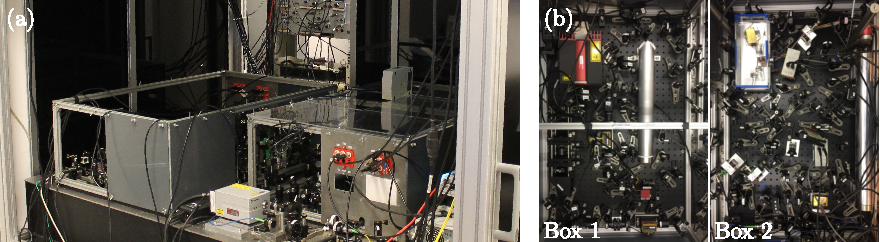
\includegraphics[width=\textwidth]{./chap6/fig/manipssqz.pdf}
    \caption{Pictures of the optical setup for squeezed light generation and detection. (a) Overview of the experiment inside the cabin. (b) Top view of the two boxes containing the optics for squeezed light generation and detection.}
    \label{fig:opticaltable}
\end{figure}


We first provide a general overview of the optical setup used to generate and manipulate squeezed light. 
Two lasers are used in this setup, to give flexibility as to produce bright squeezing directly from the OPO (one laser only), or produce vacuum squeezing to be mixed with a bright coherent field (two lasers). Both lasers are 1064 nm Nd:YAG lasers (Coherent Mephisto and Mephisto S) as in the previous chapter. The full optical layout is shown in Fig. \ref{fig:opticalpath}. The dashed box on the right part of the squeezing setup is the one to be changed to implement both configurations, as shown in Fig. \ref{fig:configsqueezer}. The experiment was designed to easily switch between the two configurations. Throughout this chapter, we will refer to three different optical cavities common to both configurations: the infrared mode cleaner (IRMC) cavity, the SHG cavity, and the OPO cavity. Each of these cavities is central to the generation and manipulation of squeezed light, and their characterization is detailed in the following sections. \\ 

\begin{figure}[h!]
    \centering  
    \includegraphics[width=\textwidth]{./chap6/fig/schemaSqz.pdf}
    \caption{Optical layout for squeezed light generation and detection. The setup includes two Nd:YAG lasers, an IRMC cavity for spatial filtering, a SHG cavity to produce the pump beam at 532 nm, and an OPO cavity for squeezing generation. The homodyne detection setup is used to measure the squeezed states. Key components such as electro-optic modulators (EOMs), piezoelectric transducers (PZTs), and photodiodes (PDs) used for locking and detection purposes are indicated. The dashed box on the right side represents the section that can be modified to implement different squeezing configurations, as detailed in Fig. \ref{fig:configsqueezer}.}
    \label{fig:opticalpath}
\end{figure}

To generate bright squeezed light from an OPO, we now detail the two different configurations implemented in this setup, as shown in Fig. \ref{fig:configsqueezer}. The only notable modification between the two configurations lies in the way the OPO is seeded and locked, and in what the piezo actuators are used for. 

\begin{figure}[h!]
    \centering  
    \includegraphics[width=\textwidth]{./chap6/fig/config_squeezer.pdf}
    \caption{Schematic of the two configurations for squeezed light generation. (a) Configuration I: bright squeezing from OPO using a single laser source. The IR beam from the IRMC cavity is split into two paths: one for the local oscillator (LO) and one as a bright seed for the OPO. (b) Configuration II: vacuum squeezing with a bright seed using two lasers. The first laser serves as the detection LO and bright coherent state, while the second laser provides a bright coherent field detuned from the OPO resonance. The vacuum squeezing is then mixed with the bright seed to generate bright squeezing.}
    \label{fig:configsqueezer}
\end{figure}


\subsubsection{Configuration I: Bright squeezing from OPO} The first configuration uses a single laser source, where the main laser beam is split into two paths. It is shown in Fig. \ref{fig:configsqueezer}(a). The IR beam output from the IRMC cavity is split in two paths: one path is the LO used in the detection, while the other one is sent to the OPO as a bright seed. Locking the pump phase then allows to select the squeezed quadrature. The piezo shown is then used to lock the LO phase. 

\subsubsection{Configuration II: vacuum squeezing + bright seed} The second configuration employs both lasers. Its schematic configuration is shown in Fig. \ref{fig:configsqueezer}(b). The first laser is used both as a detection LO, as well as a bright coherent state to be mixed with the squeezed vacuum generated by the OPO. In this case, the piezo shown is used to lock the the relative phase between the bright seed and the vacuum squeezing ellipse angle in order to select the squeezed quadrature. A second piezo not displayed here is used to lock the signal quadrature to be probed by the detection. The second laser provides a brigth coherent field detuned from the OPO resonance. This field, seen as a strong sideband, is injected into the OPO cavity. The photons generated from the pump beam at 532 nm will then be down-converted into pairs of photons, which eventually populate the sideband mode at the second laser frequency. These correlated photons being equally distributed in the upper and lower sidebands around the first laser frequency (since the pump was generated from it), demodulating the IR signal leaking from the cavity at the PLL frequency and twice the PLL frequency allows to extract two error signals. The first one, at the PLL frequency, gives us the phase of the pump with respect to the bright seed, while the second one, at twice the PLL frequency, gives us access to the quadrature angle of the squeezed vacuum with respect to the bright seed. Hence, we lock the pump phase using the first error signal, while the second error signal is used to lock the homodyne angle to the optimal squeezing quadrature. \\ 

The second configuration is more complex to implement, but is meant to make the squeezing generation more robust to low-frequency noises. It was studied over M. Croquette's PhD thesis \cite{croquette} and the start of mine, where we obtained 3 dB of vacuum squeezing and 1.5 dB of bright squeezing. These results will quickly be summarized in section \ref{sec:bright_squeezingII}, but we will mainly focus on the first configuration in the rest of this chapter (\ref{sec:bright_squeezingI}), as it is simpler to implement and optimize. 

\section{Cavity Resonances and Locks}

\subsection{IRMC Cavity}
The first cavity presented is the infrared mode cleaner (IRMC) cavity( see Fig. \ref{fig:opticalpath}). The purpose of this cavity is to spatially filter the laser beam, ensuring a high-quality $\text{TEM}_{00}$ mode profile, as well as \textit{cleaning} the IR beam from any excess classical noise as developped in Chapter I. It is a three-mirror travelling-wave Fabry-Perot resonator with a total round-trip length of $L = 84$ cm, corresponding to a free spectral range of $\mathrm{FSR} = 357$ MHz. The input and output couplers have a radius of curvature of $\mathrm{RoC} = -2$ m, while the middle mirror is flat. With a measured optical linewidth of $\kappa/2\pi = 52$ kHz, the finesse reaches a value of $\mathcal{F} \sim 7000$, which ensures significant filtering of laser frequency noise and intensity noise above the cavity linewidth. The associated round-trip losses are estimated to be around $900$ ppm, dominated by the input coupler transmission of $T_1 = 666$ ppm. The cavity parameters are summarized in Table \ref{tab:IRMC_params}. \\

\begin{table}[h!]
\centering
\captionsetup{width=\linewidth}
\begin{minipage}[t]{0.5\linewidth}
  \centering
  \textbf{Specifications}\par\medskip
  \begin{tabular}{lc}
    \hline
    Length (cm) & 84.0 \\
    FSR (MHz) & 357 \\
    ST\_1\_1 (ppm) & 475 \\
    ST\_2\_2 (ppm) & 475 \\
    RoC (m) & -2 \\ 
  \end{tabular}
\end{minipage}\hfill
\begin{minipage}[t]{0.5\linewidth}
  \centering
  \textbf{Measurements}\par\medskip
  \begin{tabular}{lc}
    \hline
    Finesse $\mathcal{F}$ & 6812 \\
    Linewidth (kHz) & 52 \\
    $T_1+T_2+\mathcal{L}$ (ppm) & 922 \\
    Resonant reflection $R(0)$ & 0.44 \\
    $T_1$ (ppm) & 767 \\
    $T_2+\mathcal{L}$ (ppm) & 155 \\ 
  \end{tabular}
\end{minipage}

\caption{IRMC parameter summary.}
\label{tab:IRMC_params}
\end{table}



This cavity is mounted in an aluminum housing to make it as monolitic as possible. The optimal alignment of the cavity is found by first making sure the laser beam goes through the first two mirrors without being clipped. This is most easily done by positioning an IR camera in transmission of the cavity rather than a photodiode. Once the beam is well centered on the first two mirrors, we adjust the angle of the output coupler to center the beam on the concave/second mirror. We then adjust the position of the concave mirror such that the first reflection spot coincides with the input beam on the input coupler surface. Finally, we adjust the angle of the input coupler to superpose the consecutive round-trip spots with the input beam reflected from the input coupler surface. This is most easily done in the far-field limit, where great angular precision can be achieved. A characteristic elliptic shape formed by the multiple spots appears as one converges to the optimal alignment, seen both in reflection on an IR card and in transmission on the IR camera. Once the cavity is pre-aligned, we position photodiodes in both reflection and transmission of the cavity, and scan the cavity length. One can then beam walk the input beam in order to maximise the coupling to the $\text{TEM}_{00}$ mode of the cavity, observed as the highest and narrowest resonance peak in transmission. Triggering the oscilloscope on the PZT ramp, we measure the cavity linewidth and finesse, as well as the resonant reflection to estimate the various cavity parameters. \\

The cavity is then locked using a standard PDH technique, with a preliminary side-of-fringe lock to bring the cavity close to resonance. The input beam is phase-modulated at $\Omega_\mathrm{mod}/2\pi = 21$ MHz using a free space EOM (New Focus IR 4003). The cavity length is swept, and the detected reflected beam is processed with PyRPL to generate the PDH error signal. The finesse being relatively high, we observe cavity ringing effects when scanning the cavity length resonance too quickly, as already seen in the previous chapter. The cavity length is then swept over gently at 0.5 Hz to recover the expected Lorentzian resonance peaks in reflection. \\

Once locked, the intensity noise spectra of the reflected and transmitted beam are measured in direct detection. We then renormalize the transmitted spectra by the known $R(0)$ to yield equivalent optical powers. The results are shown in Fig. \ref{fig:irmcnoise}, where we observe significant noise suppression above the cavity bandwidth (half linewidth) of $26$ kHz. This is notably seen in the attenuation of the laser relaxationd peak around $1$ MHz. However, at low frequencies, the intensity noise is amplified, most likely due to the feedback loop. Above 2 MHz, the intensity noise reaches the shot-noise level, indicating that the IRMC effectively filters classical intensity noise from the laser. At the membrane fundamental mode frequency of $\sim$ 850 kHz, the laser intensity noise is suppressed by approximately 20 dB, which is beneficial for optomechanical experiments. It does however not reach the shot noise level, indicating that further improvements in the cavity locking or laser stabilization may be necessary for optimal performance. \\

\begin{figure}[t!]
    \centering  
    \includegraphics[width=\textwidth]{./chap6/fig/NoiseIRMC.pdf}
    \caption{Noise spectra of the IRMC transmitted beam in direct detection, showing significant suppression of classical intensity noise above the cavity linewidth for an input power $P_{\rm in}=10$ mW. We show the curves for unfiltered IR beams with and without the laser noise eater on: we see the relaxation peak is significantly attenuated and shifted up in frequency when the noise eater is on. However, low-frequency noise is amplified, likely due to feedback effects. Above 2 MHz, the intensity noise reaches the shot-noise level, indicating effective filtering of classical noise by the IRMC.}
    \label{fig:irmcnoise}
\end{figure}

The IRMC beam is now directed to the homodyne detection setup to measure its noise spectrum. We lock the homodyne detector and show the spectra in Fig. \ref{fig:noiseLO}, where we observe a linear variation of the phase noise with the LO power, confirming that the detected noise is indeed shot-noise limited. The residual classical noises below 2 MHz are effectively cancelled by the HD detection, and we deduce a clearance of approximately 10 dB up to 10 MHz, which is satisfactory for squeezing measurements.

\begin{figure}[t!]
    \centering  
    \includegraphics[width=\textwidth]{./chap6/fig/NoiseLO.pdf}
    \caption{Noise spectra of the IRMC transmitted beam in homodyne detection, showing shot-noise limited behavior across the measured frequency range. The noise scales linearly with the LO power, confirming the shot noise dominance. A clearance of approximately 10 dB is observed up to 10 MHz, indicating effective suppression of residual classical noise by the homodyne detection scheme.}
    \label{fig:noiseLO}
\end{figure}


\subsection{SHG Cavity}

In order to generate a stable $532\,\mathrm{nm}$ pump beam for the OPO, we implemented and characterized a linear SHG cavity. The cavity is designed to resonantly enhance an incoming IR field at $1064\,\mathrm{nm}$, and convert it to its second harmonic at $532\,\mathrm{nm}$ using a periodically-poled lithium niobate (PPLN) crystal as the nonlinear medium. The crystal is a Covesion $1\times10\times10$ mm$^3$ MgO:PPLN SHG crystal with five different quasi-phase-matching gratings in the bulk, with poling periods ranging from $6.83\,\mu\mathrm{m}$ to $6.96\,\mu\mathrm{m}$ and apertures of 1mm$^2$. The crystal is temperature-controlled using a Covesion temperature controller to achieve optimal phase matching for SHG, with a temperature stabilized to 10 mK precision. The crystal and its oven are then positioned at the center of the SHG cavity. The cavity features two mirrors with radii of curvature -250 mm, ensuring that the crystal length is shorter than the Rayleigh range of the cavity mode, thus minimizing diffraction losses. The output coupler is HR coated for both IR and green wavelengths, while the input coupler has a transmission of 10\% at $1064\,\mathrm{nm}$ and less than 1\% at $532\,\mathrm{nm}$. These characteristics are summarized in table \ref{tab:SHG params}. It results in a theoretical cavity finesse of approximately $60$ at $1064 \, \text{nm}$, while the finesse at $532 \, \text{nm}$ would be around $1$, as no cavity buildup is neither required nor desired at this wavelength. The reflected IR and green beams are then split on a dichroic mirror before being sent to their respective detection systems, as seen in Fig. \ref{fig:shglock}(a). \\ 

\begin{table}[t!]
    \centering
    \captionsetup{width=0.55\linewidth}
    \begin{tabular}{lc}
        Specifications &  \\
        \hline
        Length (cm)              & 9 \\
        FSR (GHz)                  &  3.3\\
        Specified $T_1$ @1064nm & 10\% \\
        Specified $T_2$ @1064nm & 0.5\% \\
        Specified $T_1$ @532nm & >99\% \\
        Specified $T_2$ @532nm & <0.1\% \\
        Roc input/output (mm) & -250 \\[0.6em]
        Measurements &  \\
        \hline
        Finesse IR $\mathcal{F}$& 30 \\
        Linewidth (MHz)            & 111  \\ 
        $T_1 + T_2 + \mathcal{L}$ (ppm) & $\sim 2.10^5$  \\
    \end{tabular}
    \caption{SHG cavity parameter table summary. The specified values are taken from the PhD thesis of M. Croquette \cite{croquette}.}
    \label{tab:SHG params}
\end{table}

This cavity is first aligned without the crystal in order to identify the optimal cavity mode. After removing the input coupler, the beam is centered on the output coupler and its angle is adjusted to retro-reflect the beam back onto itself (e.g., using two irises). The input coupler is then re-inserted and aligned in order to overlap the incident beam with the retro-reflected beam from the output coupler, providing a robust pre-alignment of the cavity. The PPLN crystal is subsequently inserted and its position is adjusted to recover the cavity resonances, while a transmission photodiode is used to monitor the resonance peaks on an oscilloscope. Final coupling is optimized by beam-walking the input beam to maximize the TEM$_{00}$ coupling, identified as the highest and narrowest transmission resonance; when the infrared beam is correctly routed through one of the PPLN gratings (and not between gratings), green flashes are observed at resonance, indicating efficient SHG. Initial characterization is then performed by scanning the cavity length around resonance using a piezoelectric transducer bonded to the output coupler, while maintaining an input infrared power of approximately $100\,\mathrm{mW}$. The transmitted infrared signal is monitored on a fast photodiode (see a typical trace in Fig.~\ref{fig:shglock}(b)), showing sharp infrared resonance peaks with green output occurring only in coincidence with these resonances, consistent with SHG taking place exclusively under resonant build-up of the fundamental field. The infrared finesse is measured to be $\mathcal{F}_{\mathrm{IR}}=30$, with the discrepancy attributed to imperfect knowledge of the mirror parameters and additional intracavity losses introduced by the nonlinear medium. The input polarization is adjusted using half- and quarter-wave plates in order to maximize the generated green power, and the observed symmetry of the resonance peaks further suggests negligible birefringence in the PPLN crystal. \\ 


\begin{figure}[h!]
    \centering  
    \includegraphics[width=\textwidth]{./chap6/fig/SHGlock_sweep.pdf}
    \caption{Overview of the SHG cavity locking: (a) Schematic of the PDH lock setup used to stabilize the SHG cavity length to resonance. The temperature of the PPLN crystal is locked via a commercial temperature controller from Covesion. (b) Cavity scan at low input IR power, showing the IR resonances onto which the cavity is locked. A PDH error signal, not displayed here, is tuned in order to lock the cavity. (c) Cavity lock as seen on the oscilloscope, showing the transmitted IR power (red) and the generated green power (green). We observe a drift away from the nominal peak height, due to thermal effects in the crystal: the heating of the crystal changes the effective optical length of the cavity, hence shifting the resonance condition. This needs to be tuned by the experimenter. 
     }
    \label{fig:shglock}
\end{figure}


Modulating the input IR beam at $\Omega_\mathrm{mod} / 2\pi= 21\,\mathrm{MHz}$ using the same free-space EOM as for the IRMC cavity (New Focus IR 4003), we processed the detected IR signal into a PDH error signal suitable for locking the cavity length at resonance, with a preliminary side-of-fringe lock as usual. A typical lock trace is shown in Fig.~\ref{fig:shglock}(c), where both the transmitted IR power and the generated green power are monitored on an oscilloscope. The first striking observation is the drift of the transmitted IR and reflected green power away from their nominal peak heights. This effect is attributed to thermal effects in the PPLN crystal: upon locking, the intracavity IR power stabilizes at a relatively high intensity, leading to heating of the crystal due to residual absorption. This heating causes a change in the refractive index and physical dimensions of the crystal, thereby shifting the optimal quasi-phase matching temperature (the oven would need to be locked to a lower temperature in order to compensate for this extra optical heating). As a result, the cavity drifts away from the optimal resonance, requiring a manual tuning of the temperature setpoint to recover maximum green output. Keeping the IR power at about 200 mW, we could then scan the crystal temperature to find the optimal phase-matching condition for SHG. The results are shown in Fig \ref{fig:shgtemp}(a): we found a maximum green output of around $100\,\mathrm{mW}$ at a crystal temperature of $\sim 58^{\circ}\mathrm{C}$ for the $6.90\,\mu\mathrm{m}$ grating, sufficient to pump the OPO below threshold. The conversion efficiency usually follows a sinc-squared dependence on temperature. Due to the high IR power build-up in the cavity, thermal effects are observed, which distort the expected sinc$^2$ shape \cite{boyd}. The side lobes of the sinc$^2$ curve are seen when scanning the temperature over a larger range, but we only show the central peak here. The symmetric sinc$^2$ shape is however recovered when injecting an order of magnitude less IR power, which is irrelevant to our purpose as it does not provide sufficient power for the OPO. To measure our SHG conversion efficiency, we varied the input IR power while keeping the crystal temperature at the optimal phase-matching point by tuning the temperature slightly at each new IR power injected to maximise the output green power. The results are shown in Fig \ref{fig:shgtemp}(b), where we observe a pseudo-linear dependence of the green output power with respect to the input IR power. From a linear fit, we extract a conversion efficiency of approximately $54\%$, which is (very) satisfactory for our application, and rather high compared to similar dedicated SHG experiments \cite{Vidal25}. \\ 

\begin{figure}[t!]
    \centering  
    \includegraphics[width=\textwidth]{./chap6/fig/SHGscansTemp.pdf}
    \caption{Output power of the SHG cavity against different parameters: (a) Output green power measured vs. crystal temperature, showing the phase-matching curve at high input IR power. A hysteresis is observed due to thermal effects. (b) Output green power as a function of the IR input power, showing pseudo-linear behavior. The SHG conversion efficiency is extracted from a linear fit, yielding a value of $54 \%$.}
    \label{fig:shgtemp}
\end{figure}


We can now place a photodiode on the path of the outgoing green beam to monitor its intensity noise spectrum. The results are shown in Fig. \ref{fig:shgnoise}: we observe significant excess intensity noise above the shot-noise level for frequencies in the Hz - 10 MHz range. We identify the peak at 2 MHz as the relaxation oscillation of the IR laser transduced to the second harmonics field. This excess noise will severely limit the achievable squeezing level from the OPO, as classical pump noise is known to degrade squeezing generation. We can however expect to achieve squeezing above the 2 MHz band. \\ 

\begin{figure}[h!]
    \centering  
    \includegraphics[width=\textwidth]{./chap6/fig/NoiseSHG.pdf}
    \caption{Intensity noise spectrum of the SHG output beam, showing significant excess noise above the shot noise level across the measured frequency range. The relaxation peak at 2 MHz is notably transduced from the fundamental IR laser to the second harmonic field, indicating that classical pump noise may limit squeezing performance in the OPO. The noise floor is not the same as for the previous figure because the RBW is different. }
    \label{fig:shgnoise}
\end{figure}



We now have a \textit{clean} $\text{TEM}_{00}$ IR beam from the IRMC cavity with an output power up to 200 mW, as well as a stable $\text{TEM}_{00}$ 532nm green pump beam from the SHG cavity delivering up to 200 mW. Both beams are now directed to the OPO cavity for squeezing generation. Further improvements of the experimental setup could include a Mach-Zehnder (MZ) interferometer after the SHG cavity to stabilize the green power sent to the OPO, as thermal effects in the PPLN crystal can lead to fluctuations in the output power over time, as well as a mode cleaner cavity for the green beam too, to ensure a high-quality spatial mode and suppress classical noise from the SHG process and cavity locking. However, these improvements have not been implemented yet in the current setup.

\subsection{OPO Cavity}
The final cavity is the Optical Parametric Oscillator (OPO) cavity, which is the core of the squeezed light generation setup. The OPO is a bow-tie travelling-wave cavity designed to be resonant for both the fundamental IR field at $1064\,\mathrm{nm}$ and the pump field at $532\,\mathrm{nm}$. The cavity contains a periodically-poled potassium titanyl phosphate (PPKTP) crystal as the nonlinear medium for parametric down-conversion. The crystal is a Raicol $1\times5\times11.2$ mm$^3$ PPKTP crystal with a poling period of $9.0\,\mu\mathrm{m}$, designed for type-I phase matching at room temperature. It has been coated on both sides to be anti-reflective at both $1064\,\mathrm{nm}$ and $532\,\mathrm{nm}$ by Laseroptik, and is mounted in a temperature-controlled oven to maintain phase-matching conditions, with a temperature stability of 100 mK. The crystal further features a wedge angle on one face to allow for gross tuning of the quasi-phase-matching condition by displacing the crystal using the 4-axis mount the whole assembly is held on (Newport 9071-M). The fine tuning of the phase-matching is achieved by adjusting the crystal temperature. \\

The cavity is formed by two concave mirrors with a radius of curvature of $25\,\mathrm{mm}$, as well as two flat mirrors. One of the flat mirrors is mounted on a PZT actuator to allow for cavity length tuning and locking. The angle of the bow-tie cavity needs to be as small as possible to optimize the mode matching (reduces astigmatism), while keeping a sufficient distance between the mirrors to accommodate the crystal mount without clipping the beam. To align the cavity, we follow a similar procedure as for the IRMC cavity (and any travelling-wave cavity for that matter). Using the pump beam as a proxy (because it can be seen with the eye), we first center the beam on the first two (flat) mirrors without clipping, then adjust the angle of the second mirror to center the beam on the first concave mirror. We similarly ajust the position of this mirror to center the beam on the second concave mirror, and then adjust its angle to reflect it onto the input beam spot on the input coupler surface. Finally, we adjust the angle of the input coupler to superpose the consecutive round-trip spots with the input beam reflected from the input coupler surface, once again in the far-field limit for better precision (and watch out for that typical elliptical shape). Once the cavity is pre-aligned, we position a photodiode in both reflection and transmission of the cavity, and scan the cavity length. One can then beam walk the input beam in order to maximise the coupling to the $\text{TEM}_{00}$ mode of the cavity as usual. We then insert back the crystal mount and adjust its position to recover the cavity resonance peaks. This step can be very tricky and time-consuming, as the crystal mount can easily clip the beam if not well centered. Injecting the IR beam from the IRMC output, we then beam walk the input beam to maximize the coupling to the $\text{TEM}_{00}$ mode of the cavity. To achieve co-resonance, we then proceed to the gross tuning of the quasi-phase-matching condition by displacing the crystal laterally using the 4-axis mount while scanning the cavity length, by periodically beam walking the two beams to remain optimally matched to the fundamental mode. We can then proceed to the cavity characterization. \\

The mirror coatings of the OPO cavity were selected with the primary objective of maximizing the escape efficiency of the squeezed field at 1064\,nm, while maintaining a pump resonance at 532\,nm that is sufficiently robust for stable operation. As seen before in Chap. I, this motivates an overcoupled design at 1064\,nm, in which the desired output coupler dominates the total round-trip dissipation. Writing the effective round-trip loss rate for the down-converted field as the sum of the output coupling and parasitic losses, we recall the definition of the escape efficiency $\eta_{\mathrm{esc}}$:
\begin{equation*}
\eta_{\mathrm{esc}}
= \dfrac{\kappa_{2}}{\kappa} = \frac{T^{1064}_{2}}{T^{1064}_{2} + T^{1064}_{1} + \mathcal{L}},
\label{eq:eta_esc_def}
\end{equation*}
where $T^{1064}_{1}$ is the power transmittivity of the 1064\,nm output coupler and $\mathcal{L}$ denotes the additional loss. Experimentally, we measured $T^{1064}_{\mathrm{out}} + \mathcal{L} \simeq 7.5\%$. Assuming additional losses on the order of a few hundred ppm, we get an estimated escape efficiency of $\eta_{\mathrm{esc}} \approx 99.2\%$. \\ 

On the pump side (532\,nm), the coating strategy is intentionally different. The pump resonance was designed to be low finesse ($\mathcal{F}_{532}\approx 8.5$) with a large pump input coupler ($T^{532}_{\mathrm{in}}\approx 74\%$). A broad pump resonance improves operational robustness by reducing sensitivity to cavity-length fluctuations and simplifying acquisition and locking, while still enabling sufficient circulating pump power to reach threshold (measured $P_{\mathrm{th}}\approx 80\,\mathrm{mW}$). It however jitters the coresonance, seen as abrupt variations of the seed amplification/deamplification traces, too fast to be corrected by the temperature control. Overall, the combined coating choices implement a consistent design philosophy: \textit{minimize parasitic loss and enforce overcoupling at 1064\,nm to maximize escape efficiency and preserve squeezing}, while \textit{keeping the pump resonance forgiving and efficiently driven at 532\,nm to ensure stable, reproducible operation}. The measured parameters of the OPO cavity are summarized in Table \ref{tab:OPO params}. \\

\begin{table}[t!]
    \centering
    \captionsetup{width=0.55\linewidth}
    \begin{tabular}{lc}
        Specifications &  \\
        \hline
        Length (cm)              & 27.2 \\
        FSR (GHz)                  &  1.1\\
        RoC (mm) & -38 \\[0.6em]

        Measurements &  \\
        \hline
        IR Finesse $\mathcal{F}_{1064}$& 84 \\
        IR Linewidth (MHz)            & 13  \\
        IR resonant reflection R$^\text{1064}$(0) & 0.97 \\
        IR input coupler $T_1^{\text{1064}}$ & 0.02\%\\
        IR output coupler $T_2^{\text{1064}} + \mathcal{L}$ & 7.5\% \\[0.6em] 

        Pump Finesse $\mathcal{F}_{532}$& 8.5 \\
        Pump Linewidth (MHz)            &  130  \\
        Pump resonant reflection R$^{532}$(0) & 0.87 \\
        Pump input coupler $T_1^{532}$ & 74\% \\
        Pump output coupler $T_2^{532} + \mathcal{L}$ & 3\% \\[0.6em]

        OPO threshold P$_{\text{th}}$ & 80.2 mW \\
        escape efficiency & 99.2\% \\ 
    \end{tabular}
    \caption{OPO cavity parameter summary.}
    \label{tab:OPO params}
\end{table}



The cavity length is now swept using the PZT actuator to observe the resonances at both wavelengths. The input pump beam is phase-modulated at $\Omega_\mathrm{mod}/2\pi = 19\,\mathrm{MHz}$ (New Focus IR 4001), and the transmitted and reflected signals are manipulated with PyRPL to generate a PDH error signal suitable for locking the cavity length to resonance, with a preliminary side-of-fringe lock as usual. Once locked, we proceed to the fine-tuning of the quasi phase-matching condition by adjusting the crystal temperature to maximize the amplification/deamplification of the seed. Fig \ref{fig:oposcans}(a) shows a typical scan of the cavity length below threshold, where we observe the co-resonance of both the pump and IR beams. Above threshold, as seen in Fig \ref{fig:oposcans}(b), the IR resonance peak height increases significantly due to the onset of parametric oscillation, indicating that the pump power has exceeded the threshold value, such that IR photons are generated at every pump resonance (which is not the case below threshold). This is a clear signature of OPO operation. \\
\begin{figure}[t!]
    \centering  
    \includegraphics[width=\textwidth]{./chap6/fig/scansOPO.pdf}
    \caption{OPO resonances observed by scanning the cavity length. The green curves show the transmitted and reflected pump power and the grey curve shows the piezo ramp. The dim red curve corresponds to the transmitted IR power when pumping the OPO with the 532 nm beam (hence undergoing parametric processes), while the solid red curve shows the raw transmitted IR power (no pump). (a) Co-resonance of the pump and IR beam below threshold i.e. the beam is parametrically amplified/deamplified. (b) Resonance of the IR beam above threshold, showing the onset of parametric oscillation as the pump power exceeds the threshold value.
     }
    \label{fig:oposcans}
\end{figure}

To precisely estimate the OPO threshold power, we measure the amplified and deamplified output IR power when seeding the OPO with the IR seed. By sweeping the pump power from zero to above threshold while keeping the seed power constant, we record the extrema of the typical gain curve shown in Fig \ref{fig:ampdeamp}(a). The curve obtained is fitted using the standard OPO gain model \cite{bachor2004guide}, and we find a threshold power of $P_{\mathrm{th}} \simeq 105\,\mathrm{mW}$ for the amplification data, and $P_{\mathrm{th}} \simeq 80\,\mathrm{mW}$ for the deamplification data. \\ 
\begin{figure}[b!]
    \centering  
    \includegraphics[width=\textwidth]{./chap6/fig/ampdeamp.pdf}
    \caption{OPO characterization: (a) Measured amplified and deamplified output IR power when seeding the OPO with a coherent field (red) and varying the pump phase (grey curve). The phase of the pump is dithered to output a usable error signal to lock the pump phase (black). (b) Parametric gains vs. pump power, fitted using the standard OPO gain model to extract the threshold power.
     }
    \label{fig:ampdeamp}
\end{figure}

We then need to lock the pump phase to stabilize the squeezed quadrature angle. When seeding the OPO with a bright coherent field from the IRMC output, we detect the transmitted IR beam on a photodiode by placing a 99:1 beamsplitter and directing the 1\% port to a fast photodiode in direct detection while the 99\% port is sent to the homodyne detection setup. We implement a lock-in technique by modulating the pump phase at $\sim$ 50 kHz using the PZT mounted mirror in the pump path. The detected IR signal is demodulated with a variable phase shift to generate an error signal proportional to the derivative of the amplified/deamplified output power with respect to the pump phase. This error signal is then fed to a PyRPL PID module before seeding it back to the PZT actuator to lock the pump phase to the deamplification phase. The error signal is shown in Fig \ref{fig:ampdeamp}(a), where we observe a clear zero-crossing at the deamplification point. Once locked and optimized, we can proceed to the noise study of the resulting bright squeezed state. 
\section{Squeezed State Detection}

\subsection{Configuration I}\label{sec:bright_squeezingI}
In order to characterise the generated squeezed states from the OPO, we send the transmitted squeezed beam to the homodyne detection setup. We first calibrate the shot-noise level by blocking the OPO output beam and measuring the homodyne noise spectrum for various LO powers, as seen in Fig \ref{fig:noiseLO}. The homodyne detection is carefully balanced to ensure maximum common mode rejection of classical noises, and the LO power is set to about 10 mW for optimal clearance above the electronic noise floor, typically 10 dB in our case. The common mode rejection ratio is measured to be at least 10 dB across the measured frequency range using the attenuation of the LO intensity noise when both photodiodes are illuminated. A proper calibration of the common mode rejection ratio would be needed to be more precise (using a proper AM tone), but this is sufficient for a preliminary characterization. \\

The circuit of the homodyne detection was elaborated by L. Neuhaus in his PhD thesis \cite{neuhaus}, and features two output channels. The first one, a DC - 100 kHz output, is used to monitor the DC level of the homodyne signal, useful for alignment, mode matching optimization and locking. The second output channel is a RF output, AC coupled (0.1 - 100 MHz), which is sent to a spectrum analyser to measure the noise spectrum of the detected quadrature. The LO phase can be scanned using a PZT actuator on which one of the homodyne mirrors is glued, or locked to a specific quadrature using a lock-in technique similar to the one used for the OPO pump phase lock. Injecting the bright squeezed beam from the OPO of about 10 $\mu$W, the visibility of the detection is optimized by adjusting the LO mode matching and alignment, as well as the relative angle of the two polarizations using a half-wave plate before the PBS. A visibility of 98\% is achieved, which is satisfactory. The properties of the beam splitter used to mix the signals being very dependent both on angle and polarization, we need to carefully adjust these for the incoming beams to maximize the visibility. A trick is to slightly ellipticize the beams using a quarter-wave plate, in order to converge to the optimal balance more easily. \\ 

\begin{figure}[t!]
    \centering  
    \includegraphics[width=\textwidth]{./chap6/fig/OPOsweep.pdf}
    \caption{Noise level of the bright squeezed beam from the OPO while scanning the LO phase (blue), showing squeezing and anti-squeezing levels at 10 MHz analysis frequency. The shot-noise is plotted in red. We measure a squeezing level of 1.6 dB and an anti-squeezing level of about 9.0 dB. 
     }
    \label{fig:OPOsweep}
\end{figure}

 \begin{figure}[b!]
    \centering  
    \includegraphics[width=\textwidth]{./chap6/fig/OPOnoises.pdf}
    \caption{Homodyne noise spectra of the 10 $\mu$W bright squeezed beam from the OPO, showing squeezing (blue) and anti-squeezing (dark red) levels at 10 MHz analysis frequency. The squeezing level is limited at low frequencies by classical pump noise from the SHG cavity, with squeezing only observed above 5 MHz. The relaxation peaks at 1 MHz and 2 MHz are also identified, as well as the beatnote between the two modulations at 19 MHz and 21 MHz.}
    \label{fig:OPOnoises}
\end{figure}


Once optimally balanced, we seed the OPO with a pump of 60 mW, expecting a squeezing-antisqueezing level of -5.3 - 12.6 dB respectively, uncorrected for detection losses, from the standard OPO squeezing model. We then measure the noise at 10 MHz while slowly scanning the LO phase. The results are shown in Fig \ref{fig:OPOsweep}, where we observe clear squeezing and anti-squeezing levels as the LO phase is scanned. We measure a squeezing level of 1.6 dB and an anti-squeezing level of about 9.0 dB at 10 MHz. These values are rather modest, and can be attributed to several factors including residual classical pump noise from the SHG cavity, imperfect mode matching and visibility in the homodyne detection, as well as parasitic losses in the OPO cavity and detection chain. Further optimization of these parameters will lead to improved squeezing performance in future experiments. The LO phase is then locked to the squeezed quadrature using the lock-in technique described earlier, and we can proceed to the spectral analysis of the squeezing level. The resulting spectra are shown in Fig \ref{fig:OPOnoises}: we observe that the pump noise from the SHG cavity limits the squeezing level at low frequencies, with squeezing only observed above 2 MHz where the pump noise reaches the shot-noise level. We also identify the relaxation oscillation of the seed beam at 1 MHz, i.e. residual from IRMC and enhanced by the homodyne detection scheme, as well as the frequency-doubled relaxation oscillation at twice the frequency, confirming the occurence of second order nonlinear processes in the OPO cavity. \\

Further characterization of the squeezing level at various pump powers and analysis frequencies could be performed to better understand the limitations of the current setup. Placing the IRMC cavity before the SHG cavity to filter the pump beam could significantly reduce classical pump noise and improve squeezing performance at low frequencies. Additionally, implementing a mode cleaner cavity for the green pump beam could enhance spatial mode quality and further suppress classical noise contributions. That was actually the initial plan, but issues in operating the green mode cleaner cavity, possibly due to the dual wavelength (IR/green) coatings prevented us from doing so. New green coatings will be used in the upcoming green filter cavity. Overall, while the current setup demonstrates the generation of squeezed states, there is room for optimization to achieve higher bright squeezing levels suitable for sub-SQL optomechanical experiments. 


\subsection{Configuration II}\label{sec:bright_squeezingII}
We now turn to the second configuration, in which the OPO is not seeded by a bright coherent field, but rather operated in the vacuum squeezing regime. The data presented here were acquired at the end of M. Croquette's PhD thesis \cite{croquette}, and I participated in the data analysis and interpretation of the results. We briefly discuss them here for completeness, but redirect the reader to his thesis for a more detailed account. \\

\begin{figure}[t!]
    \centering  
    \includegraphics[width=\textwidth]{./chap6/fig/OPOvacuum.pdf}
    \caption{Squeezing and antisqueezing levels while varying the pump phase. These levels are obtained at 500kHz analysis frequency.
     }
    \label{fig:OPOvacuum}
\end{figure}

 In this configuration, the squeezed vacuum states generated by the OPO are directly sent to the homodyne detection setup without any bright seed. The homodyne detection is configured similarly as before, with the LO power set to about 10 mW and the visibility maximized. A coherent control field (CCF) is then needed to lock both the OPO pump phase and the LO phase to the squeezed quadrature. The CCF is a weak coherent field injected into the OPO cavity at a frequency offset of about 10 MHz from the main laser frequency. The PLL to do so has been described in \cite{croquette}, and is implemented using PyRPL. The seed is initially injected into the cavity to mode match the cavity. Then, using fiber components, we change the seed for the CCF which is now detuned by an amount of the order of the OPO bandwidth such that CCF photons do see the non-linear gain of the OPO. The OPO is then locked, and the LO phase is swept to observe the squeezing and anti-squeezing levels as seen in Fig \ref{fig:OPOvacuum}(a). We observe a squeezing level of 3 dB and an antisqueezing level of 9 dB at 500 kHz analysis frequency. 

\section{Filter Cavity Concept}
As detailed in the previous chapters, the generation of squeezed states of light alone cannot allow sub-SQL measurements of a mechanical resonator embedded within a resonant optical cavity across a broad frequency range. To achieve this, the squeezed states must be manipulated in a frequency-dependent manner to optimally reduce quantum noise at each frequency of interest. This can for example be accomplished by reflecting the squeezed states off a detuned optical cavity. \\ 

\begin{figure}
    \centering  
    \includegraphics[width=\textwidth]{./chap6/fig/imgFC.pdf}
    \caption{ (a) Aerial view of the Advanced Virgo site. (b) Picture of the filter cavity vacuum tank, housing the 285-m long Fabry-Perot cavity in parallel to the North arm of the interferometer (seen on the right of the bird's eye view). 
    }
    \label{fig:imgFC}
\end{figure}

Over the course of my PhD, I was lucky enough to collaborate with the Virgo collaboration and help characterizing the Advanced Virgo filter cavity (FC), designed to provide frequency-dependent squeezing for the Advanced Virgo gravitational-wave detector. Although drastically different in scale compared to our tabletop OPO setup, the underlying principles remain the same, and it was a great opportunity to gain insight into the challenges of implementing frequency-dependent squeezing in interferometers.  \\ 

This part will briefly summarize the work done on the Virgo FC, focusing on the thermal effects encountered when implementing a bichromatic lock. This work was carried out as part of the Advanced Virgo QNR group, and in collaboration with L. D. Bonavena, a Virgo PhD student at the time, and Y. Zhao. Neither extensive reviews of the optical setup nor the detailed characterization of the cavity will be provided here, as they are out of the scope of this thesis. For further details on the Advanced Virgo squeezing filter cavity and its characterization, I refer the reader to the PhD thesis of L. D. Bonavena \cite{bonavena2024quantum},as well as the associated publications \cite{bonavena2024thermal,acernese2023frequency}. \\
\subsection{Advanced Virgo Filter Cavity}

The Virgo FC aims to implement frequency-dependent squeezing in the Advanced Virgo gravitational-wave detector, enhancing its sensitivity to gravitational waves. The cavity is a 285-m long Fabry-Perot cavity located in Cascina, close to the North arm of the interferometer. The cavity is designed to provide a frequency-dependent rotation of the squeezed quadrature at about 25 Hz, where the radiation pressure noise and shot-noise contributions are equivalent for the Virgo interferometer. The FC is mounted inside a vacuum tank, and is formed by two dual coating mirrors treated by the LMA, with input mirror IR transmittivity of 562 ppm and an end mirror transmittivity of 3 ppm, leading to a finesse of about 10000 at 1064 nm, as well as a green transmittivity of both mirrors of 2.7\%, leading to a finesse of about 120 at 532 nm. The reflected IR beams are then directed towards a standard HD detection setup. A picture of the cavity tank as well as an aerial view of the Virgo site are shown in Fig \ref{fig:imgFC}. \\ 

The vacuum squeezed light source developped for Virgo is also based upon a sub-threshold OPO, though with a different geometry \cite{acernese2019increasing}. It outputs squeezing level as high as 8.5 dB down to the Hz scale. When characterizing the filter cavity, a retro-reflector used induces a stray light bump below 20 Hz i.e. scattered light coupled to seismic noises, and limits the achievable FDS squeezing level at low frequencies. It produces FDS squeezing levels of about 5 dB which is subsequently injected into the FC. The FDS curve obtained by the Virgo collaboration in 2023 is shown in Fig \ref{fig:FDSVirgo}, showing a frequency-dependent rotation of the squeezed quadrature at about 90 Hz, limited by the stray light bump at low frequencies. \\ 

\begin{figure}
    \centering  
    \includegraphics[width=\textwidth]{./chap6/fig/FDSVirgo.pdf}
    \caption{Frequency-dependent squeezing levels obtained by the Virgo collaboration in 2023, showing a rotation of the squeezed quadrature at about 90 Hz. The low-frequency squeezing level is limited by a stray light bump below 20 Hz. Although the green beam detuning is kept constant at 45 Hz, the fitted detuning of the FDS traces varies by about 20\% over time, which is attributed to various effects, including thermal ones. 
     }
    \label{fig:FDSVirgo}
\end{figure}

The setup to lock the FC involves two IR lasers, that we will refer to as the main laser and the sub-carrier laser (SC). \\


\noindent \textbf{The main laser:} The first one is an IR laser (1064 nm) at frequency $\omega_0$, which is used to pump the SHG cavity in order to generate a green beam at frequency $\omega_p = 2\omega_0$ (532 nm). This green beam is then split in two paths. The first path is used to pump the OPO cavity below threshold to generate the vacuum squeezed states at $\omega_0$. The second path is frequency-shifted using an AOM to generate a beam at frequency $\omega_p'=\omega_p + \Delta \omega_p$, phase-modulated and subsequently injected into the filter cavity for locking. Demodulation of the reflected signal generates a PDH error signal at 532 nm.  \\  

\noindent \textbf{The SC laser:} The second laser is another IR laser at frequency $\omega_0' = \omega_0 + \Delta \omega_0$, phase-locked to the main laser with an offset frequency of $\Delta \omega_0$. This SC laser is used to probe the filter cavity at IR wavelength, by injecting it into the cavity after phase modulation to generate a PDH error signal. \\ 

The two lasers are phase/frequency-locked using a PLL scheme, such that the detuning of the SC laser with respect to both the green beam and the squeezed beam is kept constant at $\Delta \omega_0$. Importantly, injecting the \textit{bright} SC laser into the setup saturates the HD detection, such that it is currently not possible to measure HD spectra with the SC laser on. 

\subsection{Lock and thermal effects}
\subsubsection{Naive GR lock}

The first locking scheme implemented for the Virgo FC involves locking the cavity length to the green beam only, using a standard PDH technique. The green beam at frequency $\omega_p'$ is injected into the cavity, and the reflected signal used for the lock. The detuning of the squeezed beam with respect to the cavity resonance is then set by adjusting the frequency offset $\Delta \omega_p$ introduced by the AOM. To circumvent the issue of the stray light bump at low frequency, the detuning was set to 180 Hz, where the squeezing level is not significantly affected. The reflected FDS beam is then directed towards the HD detection. The LO is derived from the main laser, and the homodyne detection is performed similarly as described in section \ref{sec:bright_squeezingI}. By scanning the LO phase and recording the AC noise spectrum, the squeezing levels can be measured and the optimal LO phase can be locked. \\

Operating this setup for tens of hours (even days), it was observed that the squeezing minima drifted over time, with a characteristic period of about 24 hours. A typical trace of such a drift with both the FC and the HD angle locked (at a $\pi/2$ phase) over more than ten hours is shown in Fig \ref{fig:driftT}. The clear drift of the FDS minimum over time, points towards bichromatic detuning of the filter cavity. Recording the temperature of both cavity mirrors continuously, it was realized that these detuning drifts were correlated with temperature fluctuations of the end mirrors, as shown in Fig \ref{fig:variationT}. This effect was attributed to thermal effects, and notably to a sensitive change in the phase picked up by both beam upon reflection on the end cavity mirror (the 3 ppm one), changing the effective optical length of the cavity as seen by both wavelengths. This effect was further confirmed by performing controlled temperature variations of the end mirror, and measuring the corresponding variations in cavity detuning. 

\begin{figure}
    \centering  
    \includegraphics[width=\textwidth]{./chap6/fig/driftT.pdf}
    \caption{Observation of thermally-induced detuning drifts over time, correlated with temperature fluctuations of the end cavity mirror. The data were recorded on the 11th of January 2023. (top) FDS HD traces recorded over more than 10 hours, showing the drift of the squeezed quadrature minimum (red) with respect to the shot noise level (white). Blue areas indicate antisqueezing regions. (bottom) Temperatures of the input (green) and end (red) cavity mirrors over the same time period. }
    \label{fig:driftT}
\end{figure}



\begin{figure}
    \centering  
    \includegraphics[width=\textwidth]{./chap6/fig/variationT.pdf}
    \caption{Frequency at which strongest squeezing is detected, vs. FC end mirror temperature for the same data batch, showing a clear correlation between temperature variations and detuning drifts.}
    \label{fig:variationT}
\end{figure}

\subsubsection{Bichromatic lock}

To circumvent these thermal effects, a more robust locking scheme was implemented, relying on bichromatic locking of the cavity to both the green beam and the SC laser. This scheme ensures that the cavity remains at coresonance for both wavelengths, thereby stabilizing the detuning of the squeezed beam with respect to the cavity resonance. Both the SC laser at $\omega_0'$ and the green beam at $\omega_p'$ are injected into the cavity to achieve coresonance. Upon coresonance, the squeezed beam would be locked at the right detuning, since its detuning with respect to the SC beam is set by the PLL. The green beam at frequency $\omega_p'$ is once again obtained by frequency shifting the green beam generated from the main laser using the AOM. The AOM is driven by a VCO, and the name of the game is to lock the VCO frequency by adjusting the seeded offset voltage. The cavity being continuously locked to the green beam while changing the VCO offset, the correct VCO offset yields coresonance. The error signal being fed back to the VCO is therefore the SC PDH error signal, which monitors the detuning of the cavity with respect to the SC laser. The PID controller output seeking to minimize this error signal is then used to adjust the VCO offset voltage, thereby locking the cavity to coresonance. The schematic of the locking setup is shown in Fig \ref{fig:bichromatic_lock}. \\ 

Thermally induced bichromatic detuning of the cavity was then further confirmed operating this setup for a long period of time upon forced temperature variations of the end mirror. The probe of this detuning over time is now the seeded VCO voltage, which directly indicates the detuning of the cavity with respect to the SC laser. We refer the reader to the associated publication \cite{bonavena2024thermal} for further details on this locking scheme and an extensive analysis of the thermal effects encountered. \\

\begin{figure}
    \centering  
    \includegraphics[width=\textwidth]{./chap6/fig/bichromatic lock.pdf}
    \caption{ Full schematic of the bichromatic locking scheme implemented for the Virgo filter cavity. The cavity length is locked to the green beam using a standard PDH technique, while the VCO offset frequency is adjusted using the SC PDH error signal to achieve coresonance for both wavelengths. The \textit{naive} lock presented in the main text is done by simply locking the cavity length to the green beam only (no PID block on the AOM). }
    \label{fig:bichromatic_lock}
\end{figure}

\subsection{Tabletop Filter Cavities}

We now briefly discuss how to implement a similar filter cavity for our prospective fibered cavity. We set the FC length at $L_{\mathrm{FC}} = 50$ cm, and consider realistic tabletop parameters of a fibered optomechanical cavity i.e. $m=10$ ng, $\Omega_m/2\pi = 1$ MHz, $Q_m = 10^6$, $\mathcal{F}=1\,000$, $L=500$ $\mu$m and $P_\mathrm{in} = 100$ $\mu$W. The optomechanical cavity bandwidth $\kappa/2\pi = \omega_{\rm{FSR}}/\mathcal{F}= 300$ MHz such that we sit in the unresolved sideband regime, while the mechanical bandwidth is about 1 Hz. We then compute the required filter cavity linewidth as seen in Chap. II as 
\begin{equation}
\begin{split}
\kappa_{\mathrm{FC}} & = \Gamma_m \dfrac{1 - |\mathcal{K}(\Omega_m)|^2}{|\mathcal{K}(\Omega_m)|}\\ 
& \sim 16 \,\mathrm{kHz}
\end{split}
\end{equation}
where $\mathcal{K}(\Omega)$ is the optomechanical coupling factor defined in Eq. (\ref{eq:K}). The corresponding finesse and input mirror transmittivity are then
\begin{equation}
 \mathcal{F}_{\mathrm{FC}} = \dfrac{\pi c}{L_{\mathrm{FC}} \kappa_{\mathrm{FC}}} \sim 18\,530, \quad T^{\mathrm{FC}}_{\mathrm{in}} = \dfrac{\pi}{\mathcal{F}_{\mathrm{FC}}} \sim 335 \,\mathrm{ppm}
\end{equation}
Such a cavity is then well within reach of current coating technologies, and could be implemented in the future to provide frequency-dependent squeezing for sub-SQL measurements of a mechanical resonator embedded within a fibered optomechanical cavity. Furthermore, as seen in Chap. II, three-mirror filter cavities could be implemented to provide an additional degree of freedom to \textit{tune} the filter cavity linewidth when accounting for losses or input power change (which changes the optomechanical coupling factor $\mathcal{K}(\Omega)$, hence the required filter cavity linewidth). This avenue is explored by several groups in the context of gravitational wave detectors \cite{stevens,ding2025}, but has remained fairly elusive to tabletop experiments so far. \\

Bichromatic locking of the filter cavity could be implemented similarly as for the Virgo FC, by using a auxiliary laser frequency-locked (PLL) detuned from the main laser. Our mechanical resonator being at MHz frequencies, the required detuning would be of the order of a few MHz, which is easily achievable using standard AOMs. Thermal effects could be less critical in this case, given the smaller power levels involved and the reduced cavity length, but should still be taken into account when designing the locking scheme. If negligible, a simpler locking scheme relying on locking the cavity to a detuned green beam could be implemented. Dual coatings for both wavelengths would however need to be carefully designed to achieve the desired finesse and linewidth at both wavelengths. Overall, implementing a filter cavity for frequency-dependent squeezing in a tabletop optomechanical setup is feasible with current technologies. 

\section{Conclusion}
In this chapter, we have presented the design, implementation, and characterization of a various cavities used in our squeezed light source, including the IRMC, SHG and OPO cavities. We have discussed and presented both configurations the setup can operate in, namely bright squeezing and vacuum squeezing regimes. The generated bright squeezed states were characterized using homodyne detection, revealing squeezing levels limited by classical pump noise and detection inefficiencies. We also explored the concept of filter cavities for frequency-dependent squeezing, and discussed its feasibility in the context of our prospective fibered MATE cavity. \\ 

Future work will focus on optimizing the squeezing levels by addressing the identified limitations, such as implementing mode cleaner cavities for both the IR and green beams to reduce classical noise contributions. Additionally, the design and implementation of a tabletop filter cavity for frequency-dependent squeezing will be pursued, leveraging the insights gained from the Virgo FC experience i.e. a tabletop implementation of bichromatic locking schemes. 



\chapter*{Summary, conclusion and perspectives}
This chapter will cover the summary of the work done, the conclusions drawn from the experiments, and the perspectives for future research in optomechanical systems. It will highlight the key findings, their implications for quantum optics, and potential directions for further exploration.
% !TeX encoding = UTF-8
% !TeX spellcheck = fr_FR
% !TeX root = mythesis.tex
\chapter{Un appendice}

I'll write something here.
%%%%%%%%%%%%%%%%%%%%%%%%%%%%%% FINAL PAGES %%%%%%%%%%%%%%%%%%%%%%%%%%%%%%%%%%
\backmatter\ 
%%%%%%%%%%%%%%%%%%%%%%%%%%%%  BIBLIOGRAPHY %%%%%%%%%%%%%%%%%%%%%%%%%%%%%%%%%%
\cleardoublepage\ 
\phantomsection\ 
% \addcontentsline{toc}{chapter}{Bibliography}
%%%%% use of BiBTeX:
\printbibliography[heading=bibintoc]
%%%%% to be replaced by,  for final version:
%\intput{mythesis.bbl}
%%%%%%%%%%%%%%%%%%%%%%%%%  4th COVER %%%%%%%%%%%%%%%%%%%%%%%%%%%%%%%%%%%%%%%%
\backcover\ % requires thcover.sty loaded and thcoverdata.tex filled
\end{document}